\documentclass[11pt]{article}
\usepackage[T1]{fontenc}
\usepackage[utf8]{inputenc}
\usepackage{lmodern}
\usepackage[margin=0.98in,headheight=15pt]{geometry}
\usepackage{amsmath,amssymb,amsthm,mathtools}
\usepackage{booktabs,longtable,array}
\usepackage{graphicx,microtype,xcolor,enumitem,xurl}
\definecolor{ink}{HTML}{183F58}
\definecolor{teal}{HTML}{247974}
\usepackage[colorlinks=true,linkcolor=ink,citecolor=teal,urlcolor=ink]{hyperref}
\usepackage{fancyhdr}
\pagestyle{fancy}
\fancyhf{}
\fancyhead[L]{\small Complementary powers and Gaussian polylogarithms}
\fancyhead[R]{\small ProveIt research continuation}
\fancyfoot[C]{\thepage}
\setlength{\emergencystretch}{2em}
\setlength{\parskip}{3pt}
\numberwithin{equation}{section}
\newtheorem{theorem}{Theorem}[section]
\newtheorem{lemma}[theorem]{Lemma}
\newtheorem{proposition}[theorem]{Proposition}
\newtheorem{corollary}[theorem]{Corollary}
\theoremstyle{definition}
\newtheorem{definition}[theorem]{Definition}
\theoremstyle{remark}
\newtheorem{remark}[theorem]{Remark}
\newtheorem{conjecture}[theorem]{Conjecture}
\DeclareMathOperator{\Li}{Li}
\DeclareMathOperator{\Res}{Res}
\DeclareMathOperator{\Rea}{Re}
\DeclareMathOperator{\Ima}{Im}
\newcommand{\Q}{\mathbb Q}
\newcommand{\R}{\mathbb R}
\newcommand{\C}{\mathbb C}
\newcommand{\Z}{\mathbb Z}
\newcommand{\N}{\mathbb N}
\newcommand{\ii}{\mathrm i}
\newcommand{\dd}{\,\mathrm d}
\newcommand{\src}[1]{\nolinkurl{#1}}
\hypersetup{
 pdftitle={Complementary-Power Rigidity, a Gaussian Euler-Sum Identity, and Reflected Gamma Moments},
 pdfauthor={Research continuation prepared for Vladimir Reshetnikov with OpenAI assistance},
 pdfsubject={Exact polylogarithm identities, complementary powers, and asymptotic moment expansions}}
\title{\color{ink}Complementary-Power Rigidity,\\
 a Gaussian Euler-Sum Identity,\\
 and Reflected Gamma Moments}
\author{Research continuation prepared for Vladimir Reshetnikov\\
\small with OpenAI assistance}
\date{October 10, 2026}
\begin{document}
\maketitle
\begin{abstract}
We continue the ProveIt polylogarithm manuscript and its recent research
packages. A classification theorem shows that two distinct positive
integer pairs satisfying $r^a+r^b=1$ can occur only for a root of the
reciprocal plastic number, with pairs $(d,5d)$ and $(2d,3d)$. It gives
the sharp bound of twelve ordered solutions of $x+y=1$ inside the signed
cyclic group $\{\pm r^k:k\in\mathbb Z\}$ and an effective degree bound
for an exhaustive search. Classical functional equations then prove the
manuscript's plastic dilogarithm and trilogarithm identities and give
further identities without logarithmic terms.

We also prove the manuscript's weight-five Gaussian $S_4$ identity by
an exact rational certificate built from double shuffle, distribution,
and one explicit M\"obius path duality. The certificate is independently
replayable and does not use numerical integer-relation evidence as a
proof. On the analytic side, we determine the exponential cancellation
rate and first correction for alternating harmonic polylogarithms at
proportional depth, and prove meromorphic continuation, finite-order
asymptotics, late-coefficient asymptotics, and an explicit growing-order
remainder bound for reflected log-gamma moments. A finite identity among
their residues and a formal proof of a recorded log-sine coefficient
conjecture complete the development. We state the exact scope of each
result, document proposed manuscript corrections, and formulate further
questions. No numerical period independence or general maximal ladder
weight is claimed.
\end{abstract}
\newpage
{\fontsize{9.5pt}{11pt}\selectfont\setlength{\parskip}{0pt}\tableofcontents}
\newpage
\section{Scope, prior work, and the proved contributions}
\label{sec:scope}

The source manuscript is \emph{Polylogarithms and their Arithmetic
Bridges}, in the directory
\src{Analysis/Polylogarithms/docs/manuscript} of ProveIt
\cite{repoManuscript}. We fixed the inspected revision at
\begin{center}
\small\src{d00eba30c1ce73ee5cfbeb50bde9095246b9c25c}.
\end{center}
That revision contains the consolidated manuscript, its earlier reports,
and four relevant incoming archives. The present article is an additional
research contribution prepared for integration; it is not a replacement
for the whole manuscript or a certification of every historical claim.

The immediately preceding reports have already proved Gaussian double
parity formulas, the weight-five shuffle relation, several one-index-two
multiple-polylogarithm reductions, and the cubic and quartic
complementary-power trilogarithm examples. They also reduce the four
same-point weight-five Gaussian coordinates to at most two modulo
specified single-value products. We use those facts where appropriate
and do not count their rederivation as a new contribution. In particular,
the first follow-up problem in the exact-reductions package is the
specific $S_4$ relation proved below; its fifth asks for a classification
of complementary-power redundancies \cite{repoExact}.

\subsection{A precise contribution ledger}

\begin{longtable}{@{}>{\raggedright\arraybackslash}p{0.28\textwidth}>{\raggedright\arraybackslash}p{0.66\textwidth}@{}}
\toprule
Result & Mathematical content and proof status\\
\midrule\endhead
Complementary-power rigidity & A complete theorem for two positive
integer exponent pairs at the same real base, obtained from Ljunggren's
trinomial theorem and a root-rotation argument. It includes equal
exponents and arbitrary common divisors.\\[3pt]
Signed cyclic seeds & Exact cardinalities $0,3,6,12$, with the case
twelve characterized; a bound $b\leq\lfloor5D/3\rfloor$ for bases of
degree at most $D$. These are statements about pure powers.\\[3pt]
Plastic ladders & Analytic proofs of two specific manuscript identities,
plus explicit dilogarithm and trilogarithm identities with no
logarithmic terms. Classical functional equations are the inputs.\\[3pt]
Gaussian $S_4$ & A proved identity with a finite exact certificate.
The new ingredient relative to the preceding attempts is an explicit
M\"obius duality relation.\\[3pt]
Proportional harmonic depth & An explicit positive, decreasing, convex
exponential rate and a computable first correction, with an all-orders
expansion uniform on compact parameter sets.\\[3pt]
Reflected gamma moments & Exact poles and residue polynomials, shifted
factorial growth, late-coefficient asymptotics, and an explicit
truncation bound.\\[3pt]
Residue and log-sine identities & An exact finite reflection identity
and an unconditional formal polynomial version of a coefficient
conjecture recorded in a 2010 author preprint.\\
\bottomrule
\end{longtable}

The classification gives a particularly useful change in how one can
search. A box of polynomial coefficients is not exhaustive, even at
fixed degree. In contrast, the exponent bound proved here supplies an
exhaustive finite search for the restricted equation $r^a+r^b=1$.
Equally importantly, it identifies exactly what this search cannot
settle: multiplicative relations involving products of many factors
$1-r^j$, additional units, or more general polylogarithm arguments are
outside its scope.

The $S_4$ proof has a different character. It is a finite calculation
with convergent iterated-integral values, using explicitly justified
single-divergence relations as well as convergent identities. Its exact certificate can be checked by
rational arithmetic. The mathematical conclusion is an equality of
the corresponding periods. It is not a proof that a computed quotient
of all supplied relations is the full space of period relations, nor
does it prove that any remaining coordinate is irreducible.

\subsection{Classical inputs and attribution}

Ljunggren's irreducibility theorem is used in the precise form recorded
by Boyd, Martin, and Thom \cite[Lemma 4.1]{BoydMartinThom2015}; Tverberg's
proof is another primary reference \cite{Tverberg1960}. Rogers' pentagon
and Kummer's trilogarithm equation are classical; the modified
trilogarithm normalization and its functional equations are taken from
Zagier \cite{ZagierPolylogs1991}. The shuffle and stuffle laws and their
regularization belong to the established theory of multiple
polylogarithms \cite{jqzhao2010,PanzerParity}. The general existence
of parity reductions is therefore not being claimed here as new.

The analytic calculations use standard Mellin continuation, Lagrange
inversion, and Laplace asymptotics. What is derived is their explicit
application to the stated families, including normalization constants,
finite coefficient identities, and error terms. Mixed reflected
log-gamma moments were already introduced by Amdeberhan and coauthors
\cite{ACEMKM}; neither their definition nor their reflection symmetry
is a new observation. Their large-exponent and late-coefficient
behavior is the subject of the later sections.

This article establishes the statements it proves without asserting
first discovery in the entire literature. Exact priority for equivalent
normalizations of special-value identities is a separate bibliographic
question. The useful distinction is between proved results, numerical
checks of those results, and questions that remain open.

\subsection{Conventions}

For positive integers $s_1,\ldots,s_d$, our multiple polylogarithm uses
decreasing indices:
\begin{equation}\label{eq:mpl-convention}
 \Li_{s_1,\ldots,s_d}(z_1,\ldots,z_d)
 =\sum_{n_1>\cdots>n_d\geq1}
 \frac{z_1^{n_1}\cdots z_d^{n_d}}
 {n_1^{s_1}\cdots n_d^{s_d}}.
\end{equation}
Boundary values are assigned by the ordinary convergent series or by
the explicitly stated regularization. The corresponding hyperlogarithm
uses $dt/(t-a)$ and an outer-first word, so its integration simplex is
$0<t_N<\cdots<t_1<1$. The word letters associated to
\eqref{eq:mpl-convention} are reciprocal \emph{prefix} products.
These choices are essential to the signs in the Gaussian certificate.

All logarithms in the real algebraic and gamma sections are real
logarithms of positive numbers. Complex arguments in the Gaussian
section are connected to their convergent series, fixing the branches.
We write $G=\beta(2)$ for Catalan's constant and
$\beta(s)=\sum_{j\geq0}(-1)^j/(2j+1)^s$. The letter $h$ denotes
harmonic depth in Section~\ref{sec:saddle}; the fixed reflected exponent
in the gamma section is $m$. Repeated use of an auxiliary symbol in a
later, explicitly defined family does not identify the corresponding
constants across sections.

% Contribution for the continuing Polylogarithms report.
% Requires amsmath, amssymb, amsthm, booktabs, hyperref.
% Citation keys: Ljunggren1960, Tverberg1960, BoydMartinThom2015,
% AartsFokkinkKruijtzer2001.

\section{Rigidity of complementary powers}
\label{sec:complementary-rigidity}

The earlier complementary-power ladder starts from a relation
$r^a+r^b=1$, where $0<r<1$ and $a,b$ are positive integers.
That construction raises a concrete completeness question: can one base
have many different pairs of complementary powers?  We settle this
question for pure powers, including arbitrary common divisors in the
exponents.  The decisive arithmetic input is a classical irreducibility
theorem for trinomials.  Our conclusions concern this precisely specified
class of seeds; they do not classify general multiplicative relations
among $1-r^k$, or bound the maximum weight of polylogarithm ladders.

For $0<r<1$, define
\[
\mathcal C(r)=\{(a,b)\in\mathbb Z_{>0}^2:
                 a\le b,\ r^a+r^b=1\}.
\]
Let $\omega$ be the unique root in $(0,1)$ of
$X^3+X^2-1$.  Thus $\omega$ is the reciprocal of the plastic number.

\begin{theorem}[Complete classification of collisions]
\label{thm:complement-collisions}
For every real $0<r<1$, the set $\mathcal C(r)$ has at most two elements.
It has two elements if and only if $r^d=\omega$ for some positive
integer $d$, in which case
\[
\mathcal C(r)=\{(d,5d),(2d,3d)\}.
\]
If $\mathcal C(r)$ contains $(a,a)$, then
$\mathcal C(r)=\{(a,a)\}$ and $r=2^{-1/a}$.
\end{theorem}

The theorem supplies an exact answer to the seed-classification question
posed after the earlier cubic and quartic ladder certificates.  It is
proved below as a consequence of the Ljunggren--Tverberg theorem, with
all additional arguments included.  We make no claim that this
consequence is globally new in the literature.  The related theorem of
Aarts, Fokkink, and Kruijtzer classifies the two morphic numbers, by
requiring both $p+1$ and $p-1$ to be powers of $p$; their proof also uses
trinomial irreducibility \cite{AartsFokkinkKruijtzer2001}.  Our formulation
permits arbitrary positive exponent pairs and explicitly handles power
substitutions.

\subsection{The irreducibility input and the entire cyclotomic factor}

For $1\le a<b$, put $d=\gcd(a,b)$, $A=a/d$, $B=b/d$, and
\[
F_{a,b}(X)=X^b+X^a-1.
\]
The following precise specialization is the arithmetic input.

\begin{theorem}[Ljunggren--Tverberg, specialized]
\label{thm:trinomial-input}
The polynomial $F_{a,b}$ has exactly one irreducible factor over
$\mathbb Q$ whose roots are not roots of unity.  Its other factor is
\[
C_{a,b}(X)=
\begin{cases}
 X^{2d}-X^d+1,&(A,B)\equiv(1,5)\text{ or }(5,1)\pmod6,\\
 1,&\text{otherwise}.
\end{cases}
\]
In particular $H_{a,b}=F_{a,b}/C_{a,b}$ is irreducible, monic,
and has constant term $-1$.  Moreover
$H_{a,b}(X)=H_{A,B}(X^d)$.
\end{theorem}

This is the trinomial result of Ljunggren and Tverberg
\cite{Ljunggren1960,Tverberg1960}; a modern explicit formulation,
including the assertion that $H_{A,B}(X^d)$ remains irreducible, is
Boyd--Martin--Thom, Lemma~4.1(a),(b) \cite{BoydMartinThom2015}.
Only the trinomial theorem is used.  Its separate quadrinomial analogue
has a more delicate history and plays no role here.

For clarity, the displayed cyclotomic factor can be obtained directly,
without relying on a table of sign cases.  Suppose $|z|=1$ and
$z^a+z^b=1$.  The two unit vectors must be the two numbers
$e^{i\pi/3}$ and $e^{-i\pi/3}$, in either order.  If $w=z^d$, then
$w^A$ and $w^B$ are these primitive sixth roots.  A Bezout identity for
$A,B$ implies $w^6=1$, and $w^A$ of order six then implies that $w$
itself has order six.  Consequently $A,B$ have opposite residues
$1,5$ modulo six.  Conversely those residues make every root of
$X^{2d}-X^d+1$ a root of $F_{a,b}$.  These roots are simple: a common
zero of $F_{a,b}$ and its derivative on the unit circle would give
$a|z^a|=b|z^b|$, hence $a=b$, a contradiction.  Thus the formula for
$C_{a,b}$ accounts for the \emph{entire} cyclotomic factor.  The
remaining assertion, irreducibility of $H_{a,b}$, is the cited theorem.

\subsection{A conjugate-rotation invariant}

\begin{lemma}[The common divisor is intrinsic]
\label{lem:intrinsic-gcd}
Suppose $r^a+r^b=r^c+r^e=1$, where $0<r<1$,
$1\le a<b$, and $1\le c<e$.  Then
\[
\gcd(a,b)=\gcd(c,e).
\]
\end{lemma}

\begin{proof}
Set $d=\gcd(a,b)$.  Since $0<r<1$, it is not a root of unity, so
its minimal polynomial is $H_{a,b}$.  Theorem~\ref{thm:trinomial-input}
shows that this polynomial is a polynomial in $X^d$.  If $\zeta$ is a
primitive $d$th root of unity, $r\zeta$ is therefore a conjugate of $r$.
The second equation also holds at this conjugate:
\[
r^c\zeta^c+r^e\zeta^e=1.
\]
Taking absolute values gives equality in the triangle inequality,
because $r^c+r^e=1$.  Both summands must have the argument of their
positive real sum.  Thus $\zeta^c=\zeta^e=1$, proving
$d\mid\gcd(c,e)$.  Interchanging the pairs proves the reverse
divisibility.
\end{proof}

This step prevents a gap that would arise from normalizing the two
pairs independently.  The cyclotomic factor can have degree $2d$,
so a degree comparison before proving that the common divisors agree
would not suffice.

\subsection{The primitive coefficient comparison}

\begin{proof}[Proof of Theorem~\ref{thm:complement-collisions}]
First suppose an equal pair occurs.  Then $r^a=1/2$, so $r$ cannot
be an algebraic integer: otherwise the rational number $r^a=1/2$
would be an algebraic integer.  Any unequal pair would make $r$ a
root of the monic integer polynomial $F_{c,e}$, a contradiction.
There is only one equal pair because the powers of $r$ strictly
decrease.

Now suppose two distinct unequal pairs occur.  By
Lemma~\ref{lem:intrinsic-gcd} they have a common gcd $d$.
Replace $r$ by $r^d$ and divide all four exponents by $d$.
Both pairs are now primitive.  Their trinomials have the same
irreducible noncyclotomic factor, and their cyclotomic factors belong
to $\{1,\Phi_6\}$, where $\Phi_6=X^2-X+1$.
If the two cyclotomic factors agree, the trinomials agree, contrary
to distinctness.  After interchanging them if necessary, there must
therefore be a polynomial identity
\begin{equation}
(X^2-X+1)(X^n+X^m-1)=X^{n+2}+X^k-1,
\quad 1\le m<n,\quad 1\le k<n+2.
\label{eq:primitive-collision-factor}
\end{equation}
The coefficient of $X^{n+1}$ on the left is $-1$ unless
$m=n-1$, in which case it is zero.  The right-hand coefficient is
zero or one.  Hence $m=n-1$, and the identity reduces to
\[
X^{n+2}+X^{n-1}-X^2+X-1=X^{n+2}+X^k-1.
\]
For $n=2$ the remaining polynomial is $2X-X^2$, which is not a
monomial.  For $n>3$ its coefficient at $X^2$ is $-1$.
Thus $n=3$, which gives $m=2$ and $k=1$.
The common factor is $X^3+X^2-1$, and the two normalized pairs are
$(1,5)$ and $(2,3)$.  Conversely,
\[
X^5+X-1=(X^2-X+1)(X^3+X^2-1)
\]
shows that these two pairs do occur at $\omega$.
Finally, a third pair would have to be the same exceptional companion
of either existing pair, so no third pair occurs.
\end{proof}

\subsection{All signed pure-power unit equations}

The functional equations for polylogarithms use signs and inverses as
well as positive powers.  The preceding classification automatically
controls all such complementary arguments.

\begin{corollary}[Sharp signed-unit count]
\label{cor:signed-unit-count}
Let $\Gamma_r=\{\pm r^k:k\in\mathbb Z\}$ and
\[
\mathcal U(r)=\{x\in\Gamma_r:1-x\in\Gamma_r\}.
\]
Then $|\mathcal U(r)|$ is one of $0,3,6,12$.
For every unequal pair $(a,b)\in\mathcal C(r)$, its contribution is
the six-element set
\begin{equation}
\left\{r^a,r^b,r^{-a},r^{-b},-r^{b-a},-r^{a-b}\right\}.
\label{eq:six-unit-orbit}
\end{equation}
These sets are disjoint for different unordered pairs.
An equal pair contributes precisely $\{1/2,2,-1\}$.
The case $|\mathcal U(r)|=12$ occurs exactly when $r^d=\omega$
for some positive integer $d$.
\end{corollary}

\begin{proof}
The transformations $x\mapsto1-x$ and $x\mapsto1/x$ preserve
$\mathcal U(r)$.  For example,
$1-1/x=-(1-x)/x\in\Gamma_r$ whenever $x,1-x\in\Gamma_r$.
Their orbit consists of
\[
x,\quad1-x,\quad x^{-1},\quad(1-x)^{-1},
\quad x/(x-1),\quad(x-1)/x.
\]
Every real orbit has a representative in $(0,1)$: use $1/x$ if
$x>1$ and $1/(1-x)$ if $x<0$.  Such a representative and its
complement are $r^a,r^b$ with $a,b>0$.  The two members of a
nondegenerate real orbit that lie in $(0,1)$ are exactly $x$ and
$1-x$, so its unordered positive pair is unique.  Substituting
$x=r^a$, $1-x=r^b$ gives \eqref{eq:six-unit-orbit}.
All six entries are distinct unless $a=b$, when they reduce to
the stated three values.  The cardinalities now follow from
Theorem~\ref{thm:complement-collisions}.
\end{proof}

All four possibilities occur: $r=1/3$, $1/2$, the reciprocal golden
ratio, and $\omega$ give respectively $0,3,6,12$.
The conclusion classifies \emph{pure signed-power complements}.
It does not say that there are at most twelve useful polylogarithm
arguments: products of units $1-r^k$ can introduce many more arguments.

\begin{corollary}[Rational exponents]
\label{cor:rational-complements}
The same collision classification holds for positive rational
exponents, with the exceptional common scale $d$ allowed to be a
positive rational number.  In particular there are at most two
unordered positive rational pairs, and
\[
\#\{x\in\{\pm r^q:q\in\mathbb Q\}:1-x\in
                          \{\pm r^q:q\in\mathbb Q\}\}\le12.
\]
\end{corollary}

\begin{proof}
Given two pairs, choose a common denominator $N$ and apply
Theorem~\ref{thm:complement-collisions} to $r^{1/N}$.
A third rational pair could be included in the same denominator
and would contradict the integer theorem.  The orbit proof is
unchanged.
\end{proof}

\subsection{A provably complete bounded-degree search}

\begin{corollary}[Degree and an exhaustive exponent bound]
\label{cor:degree-search}
If $r^a+r^b=1$ with $1\le a<b$, then
\[
[\mathbb Q(r):\mathbb Q]=
\begin{cases}
b-2d,&(a/d,b/d)\equiv(1,5)\text{ or }(5,1)\pmod6,\\
b,&\text{otherwise},
\end{cases}
\qquad d=\gcd(a,b).
\]
Consequently all such bases of degree at most $D$ are found by
enumerating
\[
1\le a<b\le\left\lfloor\frac{5D}{3}\right\rfloor
\]
and retaining those whose displayed degree is at most $D$.
For primitive pairs it suffices to enumerate $b\le D+2$.
The only repeated bases in either enumeration are the classified
plastic pairs.  Equal pairs add the separate bases $2^{-1/a}$,
with $a\le D$.
\end{corollary}

\begin{proof}
The degree formula is Theorem~\ref{thm:trinomial-input}.  In the
exceptional case $b/d\ge5$, so $b-2d\ge3d$.  If the degree is
at most $D$, then $d\le D/3$ and
$b=(b-2d)+2d\le5D/3$.  The nonexceptional case is immediate.
For primitive pairs the possible degree loss is only two.
The equal-pair polynomial $2X^a-1$ has degree $a$ and is
irreducible: its reciprocal is, up to a nonzero scalar,
$X^a-2$, which is Eisenstein at $2$.
\end{proof}

This bound is sharp for infinitely many $D$: the pair $(d,5d)$
has degree $3d$ and largest exponent $5d$.
Unlike a search over bounded polynomial coefficients, the algorithm
has an explicit completeness theorem for its stated class.  No
numerical equality test is required.  A base is stored by the exact
irreducible polynomial $H_{a,b}$ together with its unique root in
$(0,1)$, and duplicate detection is exact polynomial comparison.

For illustration, the complete unequal-pair list through degree four is
\[
\begin{array}{ccl}
\text{degree}&\text{complement pair(s)}&\text{minimal polynomial}\\\hline
2&(1,2)&X^2+X-1\\
3&(1,3)&X^3+X-1\\
3&(1,5),(2,3)&X^3+X^2-1\\
4&(1,4)&X^4+X-1\\
4&(2,4)&X^4+X^2-1\\
4&(3,4)&X^4+X^3-1
\end{array}
\]
The degree-four entry with pair $(2,4)$ is exactly a square root of
the reciprocal golden ratio.  Its presence illustrates why normalization
of exponents is necessary when counting bases rather than primitive
seed types.

The exact enumeration in the accompanying certificate gives:
\[
\begin{array}{c|rrrrrrrrrrrr}
D&1&2&3&4&5&6&7&8&9&10&11&12\\\hline
\text{unequal-pair bases}&0&1&3&6&10&15&20&27&37&46&56&67\\
\text{primitive bases}&0&1&3&5&9&11&16&20&28&32&42&46\\
\text{all bases}&1&3&6&10&15&21&27&35&46&56&67&79
\end{array}
\]
Each row counts bases of degree at most $D$.  A primitive base has
an unequal complementary pair of gcd one; the intrinsic-gcd lemma
makes this definition independent of the choice of pair.
The last row also includes the $D$ equal-pair bases $2^{-1/a}$,
$1\le a\le D$.

\subsection{An exact counting formula}

The classification also counts bases without constructing or factoring
their minimal polynomials.  For $n\ge1$ define
\[
e(n)=\#\{a:1\le a<n,\ \gcd(a,n)=1,
            \ (a,n)\equiv(1,5)\text{ or }(5,1)\pmod6\}.
\]
In particular $e(n)=0$ unless $n\equiv1$ or $5\pmod6$,
and $e(1)=0$.

\begin{corollary}[Counting all bases by algebraic degree]
\label{cor:base-count}
Let $N(D)$ be the number of real $0<r<1$ with
$[\mathbb Q(r):\mathbb Q]\le D$ and $\mathcal C(r)\ne\varnothing$.
For every positive integer $D$,
\begin{align}
N(D)&=\frac{D(D+1)}2-\left\lfloor\frac D3\right\rfloor\notag\\
&\quad+\sum_{d=1}^{\lfloor D/3\rfloor}
\left\{e\!\left(\left\lfloor\frac Dd\right\rfloor+1\right)
       +e\!\left(\left\lfloor\frac Dd\right\rfloor+2\right)\right\}.
\label{eq:exact-base-count}
\end{align}
In particular,
\[
N(D)=\frac12D^2+O(D\log D),\qquad D\longrightarrow\infty.
\]
\end{corollary}

\begin{proof}
There are $D(D-1)/2$ unequal pairs with largest exponent at most
$D$, and their associated bases all have degree at most $D$.
A pair with largest exponent greater than $D$ can still have degree
at most $D$ only in the exceptional cyclotomic case.  Write that
pair $(dA,dB)$, where $\gcd(A,B)=1$ and the residues are opposite
$1,5$ modulo six.  The two inequalities are
\[
dB>D,\qquad d(B-2)\le D.
\]
Equivalently,
$B\in\{\lfloor D/d\rfloor+1,\lfloor D/d\rfloor+2\}$.
Since the exceptional normalized degree $B-2$ is at least three,
only $d\le D/3$ can occur.  This gives the sum in
\eqref{eq:exact-base-count}.
Every base counted twice is $\omega^{1/d}$, of degree $3d$;
there are exactly $\lfloor D/3\rfloor$ such duplicates.
Finally the $D$ equal-pair bases are distinct from all unequal-pair
bases and from each other.  This proves the exact formula.

For the asymptotic statement, use $0\le e(n)\le n$ to bound the sum
by
\[
\sum_{d\le D/3}\left(2\left\lfloor\frac Dd\right\rfloor+3\right)
\le2D\sum_{d\le D/3}\frac1d+D.
\]
The harmonic sum is $O(\log D)$, proving the claim.
\end{proof}

For an alternative exact implementation, when $n>1$ is coprime to
six, Mobius inversion gives
\begin{equation}
e(n)=\sum_{d\mid n}\mu(d)
       \left\lfloor\frac{n/d+1}{6}\right\rfloor.
\label{eq:exceptional-count-mobius}
\end{equation}
Indeed, after writing $a=dj$, the condition
$a\equiv-n\pmod6$ becomes $j\equiv-(n/d)\pmod6$ because every
unit modulo six is its own inverse.  For $t$ coprime to six,
the number of integers $1\le j<t$ in the residue class $-t$
is $\lfloor(t+1)/6\rfloor$.  Summing with $\mu(d)$ imposes
$\gcd(a,n)=1$.

% Citation keys: ZagierPolylogs1991, NakamuraShiraishi2025.

\section{Exact proofs and log-free ladders at the plastic base}
\label{sec:plastic-proofs}

The exceptional base in Theorem~\ref{thm:complement-collisions}
has two complementary pairs.  This additional structure produces
short proofs of two previously numerically supported formulas in
the manuscript, as well as log-free identities for $\zeta(2)$ and
$\zeta(3)$.

Throughout this section, $0<q<1$, $q^2+q^3=1$, and
$\lambda=\log q$.  The factorization in the preceding proof gives
\begin{equation}
1-q=q^5,\qquad1-q^2=q^3,\qquad
1-q^3=q^2,\qquad1-q^5=q.
\label{eq:plastic-complements}
\end{equation}
All logarithms used in the final identities are real.

\subsection{The dilogarithm formula: one Rogers pentagon}

Write
\[
R(x)=\operatorname{Li}_2(x)+\frac12\log x\log(1-x),
\qquad 0<x<1.
\]
The Rogers reflection and pentagon equations are
\begin{align}
R(x)+R(1-x)&=\zeta(2),\label{eq:plastic-R-reflect}\\
R(x)+R(y)&=R(xy)
 +R\!\left(\frac{x(1-y)}{1-xy}\right)
 +R\!\left(\frac{y(1-x)}{1-xy}\right).
\label{eq:plastic-R-pentagon}
\end{align}
They hold for $0<x,y<1$ and follow from the classical dilogarithm
functional equations; alternatively one can differentiate in $x$
and evaluate at $x=0$.  This real-domain formulation avoids branch
choices \cite{ZagierPolylogs1991}.

\begin{theorem}[The manuscript's plastic dilogarithm formula]
\label{thm:plastic-dilog}
\begin{equation}
\frac12\operatorname{Li}_2(q^2)-\operatorname{Li}_2(q^5)
=\lambda^2.
\label{eq:plastic-dilog-proved}
\end{equation}
\end{theorem}

\begin{proof}
Set $R_k=R(q^k)$.  At $(x,y)=(q,q^2)$ the three pentagon
arguments are
\[
xy=q^3,\qquad
\frac{x(1-y)}{1-xy}=q^2,\qquad
\frac{y(1-x)}{1-xy}=q^5.
\]
Hence $R_1+R_2=R_3+R_2+R_5$, or $R_1=R_3+R_5$.
Reflection gives $R_1+R_5=R_2+R_3=\zeta(2)$, so
$R_2=2R_5$.  Expanding the logarithmic corrections by
\eqref{eq:plastic-complements} gives
\[
\operatorname{Li}_2(q^2)+3\lambda^2
=2\operatorname{Li}_2(q^5)+5\lambda^2,
\]
as required.
\end{proof}

\subsection{The trilogarithm formula: one Kummer specialization}

For real nonzero $z\ne1$, define the single-valued trilogarithm
\[
P(z)=\operatorname{Re}\operatorname{Li}_3(z)
 -\log|z|\operatorname{Re}\operatorname{Li}_2(z)
 -\frac13\log^2|z|\log|1-z|,
\]
with the continuous value $P(1)=\zeta(3)$.
The inversion and duplication equations are
\[
P(z^{-1})=P(z),\qquad P(z)+P(-z)=\frac14P(z^2).
\]
Kummer's nine-term equation, in this single-valued real form, is
\begin{align}
&2P(x)+2P(y)
 +2P\!\left(\frac{x(1-y)}{x-1}\right)
 +2P\!\left(\frac{y(1-x)}{y-1}\right)\notag\\
&\quad+2P\!\left(\frac{1-x}{1-y}\right)
 +2P\!\left(\frac{x(1-y)}{y(1-x)}\right)
 -P(xy)-P(x/y)\notag\\
&\quad-P\!\left(\frac{x(1-y)^2}{y(1-x)^2}\right)
 =2\zeta(3).
\label{eq:plastic-Kummer}
\end{align}
We use the form recorded by Zagier, Section~7, Example~3,
equation~(7) \cite{ZagierPolylogs1991}.

The single-valued Landen equation is
\[
P(x)+P(1-x)+P(1-x^{-1})=\zeta(3),\qquad0<x<1.
\]
Its ordinary real counterpart is
\begin{align}
\operatorname{Li}_3(x)+\operatorname{Li}_3(1-x)
 +\operatorname{Li}_3(1-x^{-1})
 &=\zeta(3)+\zeta(2)\log x\notag\\
 &\quad-\frac12\log^2x\log(1-x)+\frac16\log^3x.
\label{eq:plastic-ordinary-Landen}
\end{align}
One obtains it by differentiation using dilogarithm reflection and
Landen, with the integration constant determined at $x=1$.
See also Nakamura--Shiraishi \cite{NakamuraShiraishi2025}.

\begin{theorem}[The manuscript's plastic trilogarithm formula]
\label{thm:plastic-trilog}
\begin{equation}
-\operatorname{Li}_3(q)+\frac32\operatorname{Li}_3(q^2)
 +\frac13\operatorname{Li}_3(q^3)-\operatorname{Li}_3(q^5)
=\lambda^3.
\label{eq:plastic-trilog-proved}
\end{equation}
\end{theorem}

\begin{proof}
Put $P_k=P(q^k)$.  At $(x,y)=(q,q^2)$, the nine arguments in
\eqref{eq:plastic-Kummer}, in displayed order, are
\[
q,\quad q^2,\quad -q^{-1},\quad -q^4,\quad q^2,
\quad q^{-3},\quad q^3,\quad q^{-1},\quad q^{-5}.
\]
Using inversion and duplication, the equation becomes
\[
\mathsf K=-P_1+\frac92P_2+P_3-2P_4-P_5+\frac12P_8
=2\zeta(3).
\]
Landen at $x=q$, with $1-q=q^5$, similarly gives
\[
\mathsf A=P_1+P_5-P_4+\frac14P_8=\zeta(3).
\]
Consequently the exact row operation $(\mathsf K-2\mathsf A)/3$
proves
\begin{equation}
-P_1+\frac32P_2+\frac13P_3-P_5=0.
\label{eq:plastic-P3-proved}
\end{equation}

It remains to convert this to ordinary trilogarithms.  Denote the
left side of \eqref{eq:plastic-trilog-proved} by $D$, and put
\[
S=-\operatorname{Li}_2(q)+3\operatorname{Li}_2(q^2)
 +\operatorname{Li}_2(q^3)-5\operatorname{Li}_2(q^5).
\]
The two ordinary reflection equations and
Theorem~\ref{thm:plastic-dilog} give
\begin{align*}
\operatorname{Li}_2(q)+\operatorname{Li}_2(q^5)
 &=\zeta(2)-5\lambda^2,\\
\operatorname{Li}_2(q^2)+\operatorname{Li}_2(q^3)
 &=\zeta(2)-6\lambda^2,\\
\tfrac12\operatorname{Li}_2(q^2)-\operatorname{Li}_2(q^5)
 &=\lambda^2.
\end{align*}
Taking minus the first row, plus the second, plus four times the
third yields $S=3\lambda^2$.
The remaining logarithmic coefficient in the definition of $P$ is
\[
T=\{-1\cdot1^2\cdot5
 +(3/2)\cdot2^2\cdot3
 +(1/3)\cdot3^2\cdot2
 -1\cdot5^2\cdot1\}\lambda=-6\lambda.
\]
Thus the left side of \eqref{eq:plastic-P3-proved} is
\[
D-\lambda S-\frac{\lambda^2}{3}T
=D-3\lambda^3+2\lambda^3=D-\lambda^3.
\]
This proves \eqref{eq:plastic-trilog-proved}.
\end{proof}

The proof promotes the two displayed manuscript formulas from
numerical support to exact consequences of classical functional
equations.  It does not rely on pseudointegration at an isolated
algebraic base.

\subsection{Two log-free identities}

\begin{theorem}[Log-free plastic ladders]
\label{thm:plastic-logfree}
At the same base $q$, the following identities hold:
\begin{align}
&6\operatorname{Li}_2(q)-5\operatorname{Li}_2(q^2)
 -5\operatorname{Li}_2(q^3)+6\operatorname{Li}_2(q^5)
 =\zeta(2),\label{eq:plastic-logfree2}\\
&12\operatorname{Li}_3(q)-5\operatorname{Li}_3(q^2)
 -4\operatorname{Li}_3(q^3)-8\operatorname{Li}_3(q^4)
 +8\operatorname{Li}_3(q^5)+2\operatorname{Li}_3(q^8)
 =4\zeta(3).
\label{eq:plastic-logfree3}
\end{align}
\end{theorem}

\begin{proof}
Six times the first ordinary reflection equation minus five times
the second proves \eqref{eq:plastic-logfree2}.
For the trilogarithm, write $L_k=\operatorname{Li}_3(q^k)$.
Equation~\eqref{eq:plastic-ordinary-Landen} at $x=q$ and $x=q^2$,
with duplication to eliminate negative arguments, gives
\begin{align*}
A&=L_1+L_5-L_4+\frac14L_8
  =\zeta(3)+\zeta(2)\lambda-\frac73\lambda^3,\\
B&=\frac54L_2+L_3-L_1
  =\zeta(3)+2\zeta(2)\lambda-\frac{14}3\lambda^3.
\end{align*}
The logarithmic tails are proportional.  Therefore
$4(2A-B)=4\zeta(3)$, exactly the claimed six-argument identity.
\end{proof}

These formulas are explicit additional identities for the package.
Their derivations and the classical origins of the functional
equations are given in full; no global priority claim is made.
They also give exponentially convergent algebraic series, for example
\begin{equation}
\zeta(3)=\sum_{n=1}^{\infty}
\frac{3q^n-\tfrac54q^{2n}-q^{3n}-2q^{4n}
                 +2q^{5n}+\tfrac12q^{8n}}{n^3}.
\label{eq:plastic-zeta3-series}
\end{equation}
Absolute convergence justifies expansion of the polylogarithms.
If this series is truncated after $N$ terms, its absolute tail is
at most
\[
\frac{39}{4}\,
\frac{q^{N+1}}{(N+1)^3(1-q)},
\]
obtained by summing the absolute coefficients and using
$q^{kn}\le q^n$ for $k\ge1$.  The constant $39/4$ is deliberately
simple; the sharper sum of the six individual geometric tails can
also be used.

\subsection{Exact certificates and their scope}

The accompanying script checks the polynomial identities and all
three Rogers and nine Kummer argument reductions in
$\mathbb Q[X]/(X^3+X^2-1)$.  It constructs the Kummer row from the
signed exponent list and performs the displayed rational row
operations.  Separately, it enumerates a bounded collection of
trinomials, checks the predicted cyclotomic factors and irreducible
quotients with exact polynomial arithmetic, and groups exact
minimal polynomials to verify the expected collision table.
The finite enumeration is a reproducible consistency check; the
unbounded completeness result is Theorem~\ref{thm:complement-collisions}.

\section{The mixed Gaussian weight-five conjecture is a theorem}
\label{sec:s4-proof}

Put $G=\beta(2)$ and
\[
 g_{a,b}=\operatorname{Im}\operatorname{Li}_{a,b}(i,1),
 \qquad
 S_p=\sum_{n=0}^{\infty}\frac{(-1)^nH_n}{(2n+1)^p}.
\]
The manuscript's equation \texttt{gauss:eq:S4-closed} was explicitly
classified as a numerically supported identity. We prove precisely that
identity. The contribution is a reduction of its mixed Gaussian term to
three specified single-color doubles and elementary products. It is not a
claim that the remaining doubles are independent or irreducible, nor a
claim that $S_4$ previously lacked every representation in special functions.
Indeed the 2021 discussion by Hintze and pisco already records the
representation by two colored double values and relates it to
hypergeometric evaluations \cite{hintze2021s4,mhzhao2020}.

\begin{theorem}[Certified mixed Gaussian reduction]\label{thm:s4}
With the series convention
$\operatorname{Li}_{a,b}(x,y)=\sum_{n>m\ge1}x^ny^m/(n^am^b)$,
\begin{align}
 S_4={}&\frac{4g_{4,1}-3g_{3,2}-9g_{2,3}}7
       +\frac{\pi^5}{224}
       -\frac{27}{224}G\zeta(3)-2\beta(4)\log2.
 \label{eq:s4-proved}
\end{align}
Equivalently,
\begin{align}
 \operatorname{Im}\operatorname{Li}_{4,1}(i,-1)
 ={}&-\frac{3g_{4,1}+3g_{3,2}+9g_{2,3}}7
       +\frac{\pi^5}{224}
       -\frac{27}{224}G\zeta(3)-2\beta(4)\log2.
 \label{eq:s4-mixed-proved}
\end{align}
The proof consists of convergent changes of variables, standard
shuffle/stuffle identities with the explicitly described single-divergence
regularization, and a finite rational linear combination supplied as an
independently replayable certificate.
\end{theorem}

\subsection{The arithmetic translation}
For $n=2k+1$,
\[
 H_k=\sum_{m=1}^{n-1}\frac{1+(-1)^m}{m}.
\]
Taking imaginary parts removes even $n$, while
$\operatorname{Im}(i^{2k+1})=(-1)^k$. Consequently, for $p\ge2$,
\begin{equation}\label{eq:s-harmonic-translation}
 S_p=\operatorname{Im}\left(
 \operatorname{Li}_{p,1}(i,1)+\operatorname{Li}_{p,1}(i,-1)\right).
\end{equation}
The interchange is justified by the majorant
$\sum_{n\ge2}H_{n-1}/n^p<\infty$.
Thus \eqref{eq:s4-proved} and \eqref{eq:s4-mixed-proved} are equivalent.

\subsection{A convergent octahedral change of variables}
Write $\omega_a=dt/(t-a)$ and
\[
 \mathcal I(a_1\cdots a_w)
 =\int_{0<t_w<\cdots<t_1<1}
     \omega_{a_1}(t_1)\cdots\omega_{a_w}(t_w),
\]
extended multilinearly in the letters. A convergent word has first letter
different from $1$ and last letter different from $0$.
For colors $c_j\in\mathbb Z/4\mathbb Z$, set
\[
 Z((s_1,c_1),\ldots,(s_d,c_d))
 =\operatorname{Li}_{s_1,\ldots,s_d}(i^{c_1},\ldots,i^{c_d}).
\]
Its integral word is
\begin{equation}\label{eq:s4-word-convention}
 Z(\boldsymbol s;\boldsymbol c)
 =(-1)^d\mathcal I\left(
 0^{s_1-1}i^{-c_1}\,
 0^{s_2-1}i^{-(c_1+c_2)}\cdots
 0^{s_d-1}i^{-(c_1+\cdots+c_d)}\right).
\end{equation}
This fixes both the color convention and every depth-dependent sign.

Consider the involution
\[
 \phi(t)=\frac{1-t}{1+t}.
\]
It preserves the puncture set $\{0,\infty,1,-1,i,-i\}$ and reverses the
real interval. Direct differentiation gives
\[
 \phi^*\omega_a=\omega_{\phi(a)}-\omega_{-1}\quad(a\ne-1),
 \qquad \phi^*\omega_{-1}=-\omega_{-1},
\]
where $\phi(0)=1$, $\phi(1)=0$, $\phi(i)=-i$, and
$\phi(-i)=i$. Denote this linear map on letters by $\tau$.
Changing variables and reversing the order of the simplex proves
\begin{equation}\label{eq:s4-convergent-duality}
 \mathcal I(a_1\cdots a_w)
 =(-1)^w\mathcal I\bigl(\tau(a_w)\cdots\tau(a_1)\bigr).
\end{equation}
No tangential-basepoint correction occurs here: an original last letter
other than $0$ transforms into first letters other than $1$, and an original
first letter other than $1$ transforms into last letters other than $0$.
Every term of the expansion therefore remains convergent.
The broader use of octahedral symmetries to supplement standard level-four
relations goes back to Zhao \cite{jqzhao2008,jqzhao2010}; the elementary
involution above is sufficient for the present certificate.

Only one instance of \eqref{eq:s4-convergent-duality} is needed. The word of
$\operatorname{Li}_{1,4}(i,1)$ is $(-i)000(-i)$, and hence
\begin{equation}\label{eq:s4-duality-seed}
 D:=\operatorname{Im}\left\{
 \mathcal I(e_{-i}e_0^3e_{-i})+
 \mathcal I\bigl((e_i-e_{-1})(e_1-e_{-1})^3(e_i-e_{-1})\bigr)\right\}=0.
\end{equation}
Here $e_a$ means the letter at $a$, multiplication is concatenation, and
powers are powers in the noncommutative word algebra. The transformed product expands into
exactly $32$ integral words, with coefficients $\pm1$. The first integral is
the single-color double; the second group is converted to colored
polylogarithms using \eqref{eq:s4-word-convention}.

\subsection{The standard relation rows}
The certificate uses two schemas, interpreted over $\mathbb Q$ before
imaginary parts are taken.
First, for two admissible multiple-polylogarithm index/color lists $u,v$,
let $\mathsf H(u,v)$ be the integral shuffle product and
$\mathsf S(u,v)$ the series stuffle product. Then
\begin{equation}\label{eq:s4-ds-row}
 R_{u,v}:=\operatorname{Im}\bigl(\mathsf H(u,v)-\mathsf S(u,v)\bigr)=0.
\end{equation}
The same row is used when $u=((1,0))$ and $v$ is admissible, with the standard
single-divergence regularization. This point must not be suppressed:
$\operatorname{Li}_1(1)$ itself is divergent. Its shuffle and stuffle
regularizations are both denoted by a formal variable $T$. A single leading
$(1,0)$ gives a polynomial of degree at most one in $T$, and the
regularization comparison is the identity in degrees zero and one.
Explicitly, its comparison operator satisfies
\[
 \rho(e^{Tu})=\exp\!\left(\sum_{n\ge2}\frac{(-1)^n\zeta(n)}n u^n\right)e^{Tu},
\]
so $\rho(1)=1$ and $\rho(T)=T$ \cite[Theorem~2.9]{jqzhao2010}.
Subtracting the two product expansions cancels their common divergent word
and leaves the convergent identity \eqref{eq:s4-ds-row}. This is the
single-divergence case of regularized double shuffle
\cite{racinet2002,jqzhao2010}. The verifier rejects all other divergent input
patterns and checks that every surviving word is admissible.

Second, for a list $z=((s_1,c_1),\ldots,(s_d,c_d))$ with
$c_j\in\{0,1\}$ and with all terms below convergent, ordinary distribution
is
\begin{equation}\label{eq:s4-distribution-row}
 Z(\boldsymbol s;2\boldsymbol c)
 -2^{w-d}\sum_{\boldsymbol\epsilon\in\{0,2\}^d}
 Z(\boldsymbol s;\boldsymbol c+\boldsymbol\epsilon)=0,
 \qquad w=s_1+\cdots+s_d.
\end{equation}
Indeed summing signs forces every nested summation index to be even, so the
factor is exactly $2^{w-d}$. The certificate multiplies some such relations
by an admissible value of complementary weight and expands that product by
integral shuffle. These are \emph{lifted convergent distribution} rows; no
regularized distribution formula is assumed. At weight one this includes
the elementary seed $\operatorname{Li}_1(-1)=
\operatorname{Li}_1(i)+\operatorname{Li}_1(-i)$.

\subsection{The exact certificate identity}
In the formal real vector space whose generators are imaginary parts of
convergent colored values of weight five, define
\begin{align}
 F={}&1120\operatorname{Im}\operatorname{Li}_{4,1}(i,-1)
       +480g_{4,1}+480g_{3,2}+1440g_{2,3}
       -1536\operatorname{Im}\operatorname{Li}_5(i)\nonumber\\
 &\quad+135\operatorname{Im}\bigl(\operatorname{Li}_2(i)
                                      \operatorname{Li}_3(1)\bigr)
       -2240\operatorname{Im}\bigl(\operatorname{Li}_4(i)
                                      \operatorname{Li}_1(-1)\bigr).
 \label{eq:s4-certificate-target}
\end{align}
The two products in this expression are expanded by integral shuffle.
Complex conjugation is imposed only by
$\operatorname{Im}Z(\boldsymbol s;-\boldsymbol c)
=-\operatorname{Im}Z(\boldsymbol s;\boldsymbol c)$.

\begin{lemma}[Finite rational certificate]\label{lem:s4-certificate}
The accompanying file \texttt{S4\_certificate.json} gives $911$ rational
numbers $q_r$ and $911$ standard-relation descriptors $R_r$ such that the
following is an exact equality of formal vectors:
\begin{equation}\label{eq:s4-certificate-equality}
 F=-1120D+\sum_{r=1}^{911}q_rR_r.
\end{equation}
The rows consist of $713$ convergent double-shuffle rows, $181$ rows with
one regularized weight-one factor, and $17$ lifted convergent distribution
rows.
\end{lemma}
\begin{proof}
The supplied program \texttt{verify\_s4.py} rebuilds every row from the
indices and colors in its descriptor. Integral shuffles are generated by
choosing interleaving positions, series stuffles by the three defining
recursive cases, and distribution by sign enumeration. The program also
reconstructs the single duality seed and the target independently of their
stored expansions. All coefficients are integers or instances of Python's
exact \texttt{Fraction} type. Summing the left side minus the right side of
\eqref{eq:s4-certificate-equality} yields the empty coefficient dictionary,
so every formal-word coefficient is exactly zero. The verifier neither
reruns a rank calculation nor uses numerical polylogarithms, integer-relation
searches, cached matrices, or modular arithmetic. Thus the certificate is
a finite rational proof of the stated formal equality.
\end{proof}

\begin{proof}[Proof of Theorem~\ref{thm:s4}]
Every $R_r$ vanishes by \eqref{eq:s4-ds-row} or
\eqref{eq:s4-distribution-row}, and $D=0$ by
\eqref{eq:s4-duality-seed}. The certificate therefore gives $F=0$.
Now
\[
 \operatorname{Im}\operatorname{Li}_5(i)=\beta(5)=\frac{5\pi^5}{1536},
 \qquad \operatorname{Li}_3(1)=\zeta(3),
 \qquad \operatorname{Li}_1(-1)=-\log2.
\]
Substituting these evaluations into \eqref{eq:s4-certificate-target} gives
\[
 1120\operatorname{Im}\operatorname{Li}_{4,1}(i,-1)
 +480g_{4,1}+480g_{3,2}+1440g_{2,3}
 -5\pi^5+135G\zeta(3)+2240\beta(4)\log2=0.
\]
Division by $1120$ proves \eqref{eq:s4-mixed-proved}, and
\eqref{eq:s-harmonic-translation} proves \eqref{eq:s4-proved}.
\end{proof}

\paragraph{Independent numerical audit.}
An independent real-quadrature evaluation uses
\[
 S_4=\frac16\int_0^1\frac{\log^3x\,\log(1+x^2)}{1+x^2}\,dx,
 \qquad
 g_{a,b}=\frac1{(a-1)!}\int_0^1(-\log x)^{a-1}
 \operatorname{Im}\frac{i\operatorname{Li}_b(ix)}{1-ix}\,dx.
\]
At $70$ decimal working digits it gives
\[
 S_4=-0.0104934562973350434533567510062017519635106188773197615131294,
\]
with discrepancy about $4.6\times10^{-71}$ between the two sides.
This numerical agreement is an audit of conventions, not a step in the
proof; the proof is the exact certificate above.

\paragraph{Scope and further work.}
The existing two relations among $g_{4,1},g_{3,2},g_{2,3},g_{1,4}$ may be
used to shorten \eqref{eq:s4-proved}; they are prior results and are not
counted as new here. The present proof establishes an upper bound on a
specific constant's expression complexity. It says nothing about a lower
bound, linear independence, or the impossibility of a classical-polylogarithm
reduction. A useful next problem is to compress the $911$ standard rows
into a short conceptual derivation, and to apply the same convergent
involution to the analogous odd-weight mixed sums $S_6,S_8,\ldots$.

\section{Exponential cancellation at proportional harmonic depth}
\label{sec:saddle}

The algebraic results above organize special arguments. We now turn to an
analytic question left open by the earlier alternating-harmonic report
\cite{repoHarmonic}: how rapidly does its normalized sum tend to zero
below the first-term transition? The case of proportional outer exponent
and harmonic depth has an explicit rate function. This is a continuation
of that report's results, not another proof of its already established
reflection identity.

For integers $h,n\geq0$, define
\[
 e_h(n)=[u^h]\prod_{j=1}^n(1+u/j),\qquad
 T_{p,h}(a)=\sum_{n\geq0}\frac{(-1)^ne_h(n)}{(n+a)^p},
 \quad a,p>0.
\]
Thus $e_0(n)=1$, $e_1(n)=H_n$, and
$e_2(n)=(H_n^2-H_n^{(2)})/2$. Ordinary convergence holds for $p>0$;
absolute convergence holds for $p>1$. The Gaussian normalization is
$S_{p,h}=2^{-p}T_{p,h}(1/2)$. The positive Mellin integral
\begin{equation}\label{eq:positive-mellin}
 T_{p,h}(a)=\frac{(-1)^h}{h!\,\Gamma(p)}
 \int_0^\infty
 \frac{x^{p-1}e^{-ax}\log^h(1+e^{-x})}{1+e^{-x}}\,dx
\end{equation}
follows from
\[
 \sum_{n\geq0}e_h(n)z^n
 =\frac{(-\log(1-z))^h}{h!(1-z)}
\]
by inserting an Abel factor, using the gamma integral, and taking its
limit. The exponential decay at infinity and the bound
$\log(1+e^{-x})\leq\log2$ near zero justify the integral limit.
The convergence and Abel-limit argument are also proved in
\cite[Section 3]{repoHarmonic}. In particular,
$(-1)^hT_{p,h}(a)>0$.

Put
\begin{equation}\label{eq:R-definition}
 R_{p,h}(a)=(-1)^h h!(h+a)^p T_{p,h}(a).
\end{equation}
The earlier report proves $0<R_{p,h}(a)<1$ and identifies the threshold
$p\sim h\log h$. When $p/h-\log h\to-\infty$, it proves that
$R_{p,h}(a)\to0$. The following theorem quantifies this statement when
$p/h$ remains in a fixed positive compact interval.

\subsection{The unique saddle and the rate function}

Write
\begin{equation}\label{eq:L-w}
 L(x)=\log(1+e^{-x}),\qquad
 w(x)=\frac1{(1+e^x)L(x)}=-\frac{d}{dx}\log L(x),\quad x>0.
\end{equation}

\begin{lemma}\label{lem:w}
The function $w$ is strictly increasing, with
\[
 \frac1{2\log2}<w(x)<1.
\]
For every $\alpha>0$ there is exactly one $x_\alpha>0$ satisfying
\begin{equation}\label{eq:saddle-equation}
 x_\alpha w(x_\alpha)=\alpha.
\end{equation}
Moreover $\alpha<x_\alpha<2\alpha\log2$.
\end{lemma}
\begin{proof}
Set $t=e^{-x}\in(0,1)$. Then
$w=t/((1+t)\log(1+t))$ and
\[
 \frac{d}{dt}\log w
 =\frac{\log(1+t)-t}{t(1+t)\log(1+t)}<0.
\]
Consequently $w$ increases with $x$. Its endpoint limits give the bounds.
The function $xw(x)$ has derivative $w+xw'>0$, tends to zero at zero,
and tends to infinity at infinity. This proves existence, uniqueness,
and the stated enclosure.
\end{proof}

For $x=x_\alpha$, set
\begin{align}
 \Phi_\alpha(y)&=\alpha\log y+\log L(y),\label{eq:phase}\\
 A_\alpha&=\frac{\alpha}{x^2}+w'(x)>0,\label{eq:A}\\
 I(\alpha)&=-\alpha\log(x/\alpha)-\alpha-\log L(x),\label{eq:rate}\\
 C(\alpha,a)&=
 \frac{\sqrt{\alpha/A_\alpha}}{x(1+e^{-x})}
 \exp\bigl(a(\alpha-x)\bigr).\label{eq:C}
\end{align}
All of these functions are real analytic for $\alpha>0$.

\begin{theorem}[Proportional-depth asymptotics]\label{thm:saddle}
Let $a$ and $\alpha$ range over fixed compact subsets of $(0,\infty)$,
and put $p=\alpha h$. As the integer $h\to\infty$,
\begin{equation}\label{eq:saddle-leading}
 R_{\alpha h,h}(a)
 =C(\alpha,a)e^{-hI(\alpha)}\bigl(1+O(h^{-1})\bigr),
\end{equation}
uniformly on those compact sets. In fact
\begin{equation}\label{eq:saddle-second}
 R_{\alpha h,h}(a)
 =C(\alpha,a)e^{-hI(\alpha)}
 \left(1+\frac{D(\alpha,a)}h+O(h^{-2})\right),
\end{equation}
where, with $x=x_\alpha$, $A=A_\alpha$, and
$g(y)=e^{-ay}/(y(1+e^{-y}))$,
\begin{align}
 D(\alpha,a)={}&
 \frac{g''(x)}{2Ag(x)}
 +\frac{\Phi_\alpha'''(x)g'(x)}{2A^2g(x)}
 +\frac{\Phi_\alpha''''(x)}{8A^2}
 +\frac{5\Phi_\alpha'''(x)^2}{24A^3}
 -\frac{\alpha a^2}{2}-\frac1{12\alpha}.
 \label{eq:D}
\end{align}
Every fixed further order in $h^{-1}$ exists and is effectively obtained
from derivatives of $L$ and $g$ at $x_\alpha$ and the Stirling series.
The remainder at every fixed order is uniform on the same compact sets.
\end{theorem}

\begin{proof}
Equation \eqref{eq:positive-mellin} gives
\[
 R_{\alpha h,h}(a)
 =\frac{(h+a)^{\alpha h}}{\Gamma(\alpha h)}
 \int_0^\infty e^{h\Phi_\alpha(y)}g(y)\,dy.
\]
We have
$\Phi_\alpha'(y)=\alpha/y-w(y)$ and
$\Phi_\alpha''(y)=-\alpha/y^2-w'(y)<0$.
The sole critical point is therefore a strict global maximum.
Its location stays in a fixed compact subinterval of $(0,\infty)$ as
$\alpha$ varies in the prescribed compact set, and its curvature is
bounded away from zero.

Here are explicit tail controls for the application of Laplace's method
\cite[\S2.3(iii)]{DLMFLaplace}
\cite[Section 2.3(iii)]{DLMFLaplace}. Near zero,
$\exp(h\Phi_\alpha(y))\leq y^{h\alpha}(\log2)^h$,
while $g(y)=O(y^{-1})$ uniformly in $a$. Choosing the endpoint interval
small enough makes its integral exponentially smaller than the maximum,
uniformly in $\alpha$. At infinity, $L(y)<e^{-y}$ implies
$\Phi_\alpha(y)<\alpha\log y-y$; this supplies an integrable
exponential bound uniform in the same compact parameters. On the
remaining compact set outside a fixed neighborhood of $x_\alpha$,
strict concavity and compactness give a uniform negative gap from the
maximum. These observations justify discarding both tails with an
exponentially small relative error.

In the neighborhood, substitute
$y=x+v/\sqrt h$. Taylor expansion, followed by Gaussian integration,
gives
\begin{align*}
 \int_0^\infty e^{h\Phi_\alpha(y)}g(y)\,dy
 ={}&e^{h\Phi_\alpha(x)}g(x)
 \sqrt{\frac{2\pi}{hA}}\left(1+\frac Eh+O(h^{-2})\right),\\
 E={}&\frac{g''}{2Ag}
 +\frac{\Phi'''g'}{2A^2g}
 +\frac{\Phi''''}{8A^2}
 +\frac{5(\Phi''')^2}{24A^3},
\end{align*}
with all derivatives evaluated at $x$. Odd Gaussian moments vanish;
the even moments $1/A$, $3/A^2$, and $15/A^3$ produce precisely these
four terms. The analytic functions have uniformly bounded derivatives
on a common neighborhood of the saddle. Taylor remainders there,
together with the tail bounds just given, prove the claimed uniform
error and also permit expansion to any prescribed order.

Finally Stirling's formula, uniformly for $\alpha$ in its compact set,
and $\alpha h\log(1+a/h)=\alpha a-\alpha a^2/(2h)+O(h^{-2})$
give
\[
 \frac{(h+a)^{\alpha h}}{\Gamma(\alpha h)}
 =\sqrt{\frac{\alpha h}{2\pi}}
 e^{h\alpha(1-\log\alpha)+a\alpha}
 \left(1-\frac{\alpha a^2/2+1/(12\alpha)}h+O(h^{-2})\right).
\]
Multiplying the two expansions proves
\eqref{eq:saddle-leading}--\eqref{eq:D}.
\end{proof}

\begin{remark}[Integer exponents and rounding]
For integer $p$, set $\alpha=p/h$ in the theorem. If instead one fixes
$\alpha_0$ and rounds $\alpha_0h$ to $p$, the $O(1/h)$ change of
$\alpha$ must remain inside $e^{-hI(\alpha)}$: replacing it by
$e^{-hI(\alpha_0)}$ changes the leading constant by a generally
nontrivial bounded factor. This is a practical distinction in numerical
comparisons.
\end{remark}

\subsection{Monotonicity, convexity, and matching limits}

\begin{proposition}\label{prop:rate-properties}
The rate $I$ is positive, strictly decreasing, and strictly convex on
$(0,\infty)$. More explicitly,
\begin{equation}\label{eq:rate-derivatives}
 I'(\alpha)=\log\frac{\alpha}{x_\alpha}=\log w(x_\alpha)<0,
 \qquad
 I''(\alpha)=\frac{w'(x_\alpha)}
 {w(x_\alpha)(w(x_\alpha)+x_\alpha w'(x_\alpha))}>0.
\end{equation}
Its endpoint limits are
\[
 I(0+)=-\log\log2,\qquad I(+\infty)=0.
\]
As $\alpha\to\infty$,
\begin{align}
 x_\alpha&=\alpha+\frac{\alpha}{2}e^{-\alpha}
             +O(\alpha^2e^{-2\alpha}),\label{eq:x-large}\\
 I(\alpha)&=\frac12e^{-\alpha}
      -\frac{3\alpha+5}{24}e^{-2\alpha}
      +O(\alpha^2e^{-3\alpha}),\label{eq:I-large}\\
 C(\alpha,a)&=1-
 \left(\frac{(a+1/2)\alpha}{2}+1\right)e^{-\alpha}
 +O_a(\alpha^2e^{-2\alpha}).\label{eq:C-large}
\end{align}
Also $C(\alpha,a)\to1/2$ as $\alpha\downarrow0$.
\end{proposition}
\begin{proof}
Differentiating the optimized value in \eqref{eq:rate} cancels its
$x_\alpha'$ terms by \eqref{eq:saddle-equation}. This gives the first
identity in \eqref{eq:rate-derivatives}. Differentiating
$\alpha=xw(x)$ gives the second. Positivity also follows directly:
$\log L(y)<-y$, so
\[
 \max_{y>0}\{\alpha\log(y/\alpha)+\alpha+\log L(y)\}
 <\max_{y>0}\{\alpha\log(y/\alpha)+\alpha-y\}=0.
\]
The strict inequality is valid because the first maximum is attained;
at its maximizing point the second expression is at most zero.

The small-$\alpha$ limits follow from
$x_\alpha/\alpha\to2\log2$ and
$A_\alpha\sim\alpha/x_\alpha^2$. At infinity, put $t=e^{-y}$ and use
\[
 \log L(y)=-y-\frac t2+\frac{5t^2}{24}+O(t^3),
 \qquad
 w(y)=1-\frac t2+\frac{5t^2}{12}+O(t^3).
\]
Substitution in \eqref{eq:saddle-equation} first gives
\eqref{eq:x-large}. Taylor expansion of \eqref{eq:rate} around
$y=\alpha$, retaining the quadratic displacement, gives
\eqref{eq:I-large}. Expansion of \eqref{eq:C} and
$A_\alpha=\alpha/x_\alpha^2+w'(x_\alpha)$ gives
\eqref{eq:C-large}. The remainders stated above follow from analyticity
of $\log(\log(1+t)/t)$ for $t$ near zero, with
$x_\alpha-\alpha=O(\alpha e^{-\alpha})$.
\end{proof}

The rate formula explains the scale of cancellation even when the terms
of the original alternating sum are much larger than its value. For
example, $I(1)=0.15091647898554\ldots$ and
$C(1,1/2)=0.66325765726435\ldots$. Thus
\[
 R_{h,h}(1/2)\sim0.66325765726435\ldots\,
 e^{-0.15091647898554\ldots h}.
\]
This is a proved exponential rate, rather than just a limit of zero.

The large-$\alpha$ expansions also explain why the transition parameter
in the previous report was $\lambda=he^{-\alpha}/2$. Formally putting
$\alpha=\log h+c$ in $hI(\alpha)$ gives the leading value
$e^{-c}/2$. This agrees with the independently proved transition
$R\to\exp(-e^{-c}/2)$ in \cite{repoHarmonic}. Such matching is a
consistency calculation: the compact-$\alpha$ theorem proved here does
\emph{not} by itself establish a uniform error for growing $\alpha$.
Obtaining a single effective formula across that expanding range
remains a precise further problem.

\subsection{A probability law at the saddle}

There is a useful formulation independent of the alternating series.
Normalize the positive integrand in \eqref{eq:positive-mellin}, with
$p=\alpha h$, to a probability density and call the resulting random
variable $X_h$. Then
\begin{equation}\label{eq:saddle-clt}
 \sqrt{hA_\alpha}(X_h-x_\alpha)
 \ \Longrightarrow\ N(0,1).
\end{equation}
Indeed, the same change of variables used in the proof of
Theorem~\ref{thm:saddle}, its uniform Gaussian domination on a shrinking
neighborhood, and its exponentially negligible tails prove convergence
against every bounded continuous test function. The associated rate
for $X_h$ is
$\Phi_\alpha(x_\alpha)-\Phi_\alpha(y)$.
This identifies which part of the positive integral carries the very
small alternating sum and gives a stable center for numerical quadrature.


\begin{figure}[tbp]
 \centering
 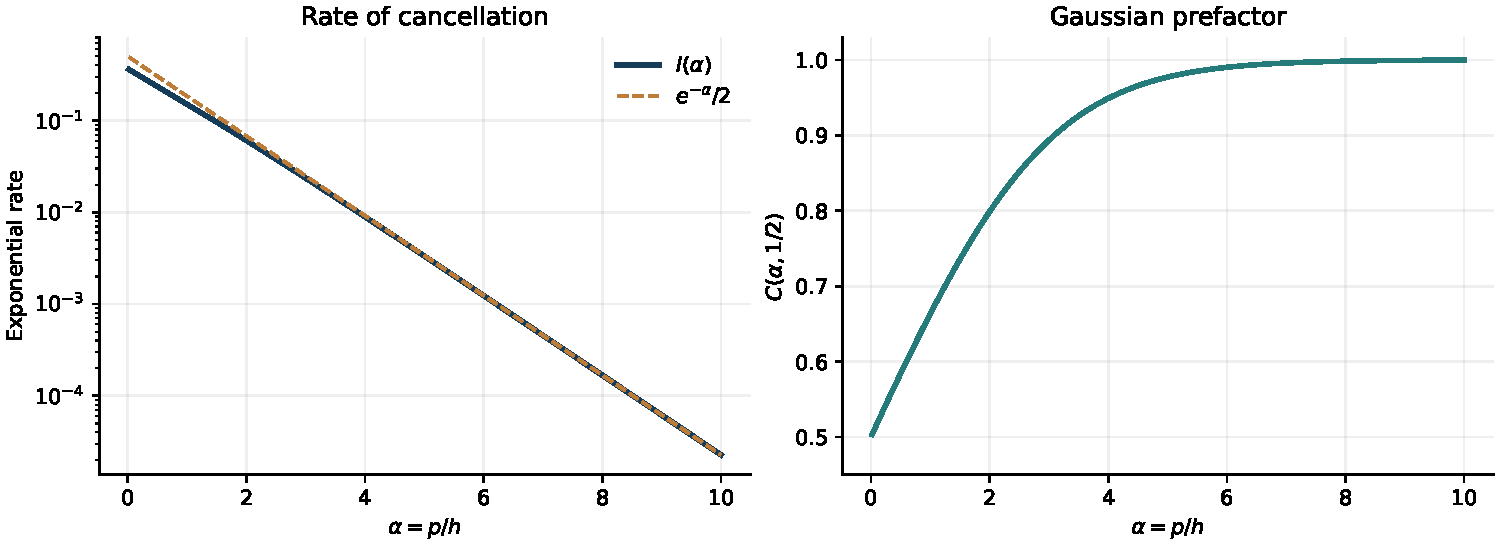
\includegraphics[width=\textwidth]{figures/saddle_rate.pdf}
 \caption{The proved rate $I(\alpha)$ and prefactor $C(\alpha,1/2)$
 from Section~\ref{sec:saddle}. The dashed curve is the leading
 large-$\alpha$ approximation $e^{-\alpha}/2$. This plot illustrates
 the exact formulas; it supplies no additional proof or error bound.}
 \label{fig:saddle}
\end{figure}
% Parent document supplies amsmath, amssymb, amsthm, and theorem environments.
% Bibliography key ACEMKM is specified in gamma_provenance.txt.
\section{Reflected log-gamma moments and their late coefficients}
\label{sec:reflected-moments}

Set $f(x)=\log\Gamma(x)$ for $0<x<1$, and define
\[
 M_{n,m}=\int_0^1 f(x)^n f(1-x)^m\,dx,
 \qquad n,m\in\mathbb Z_{\ge0}.
\]
These integrals already occur as $T_{n+m,n}$ in
Amdeberhan et al.\ \cite[Section~5]{ACEMKM}.  Their symmetry
$M_{n,m}=M_{m,n}$ and the identities obtained by expanding Euler's
reflection formula are therefore classical.  The asymptotic question here
is different: keep the reflected exponent $m$ fixed and let $n$ tend to
infinity.  The factor $f(1-x)^m$ vanishes to order $m$ at the endpoint
that produces the factorial growth.  This shifts the first exponential
scale from $1$ to $m+1$ without removing the eventual divergence of the
full expansion.  Theorem~\ref{gam:thm:late} identifies its late terms,
including their signs and the first relative correction.

\subsection{The meromorphic transform and all finite asymptotic orders}

Put
\[
 B(x)=\log\Gamma(1-x)
 =\gamma x+\sum_{j\ge2}\frac{\zeta(j)}j x^j,
 \qquad |x|<1,
\]
where $\gamma$ is Euler's constant.  For $k\ge1$ define
\begin{equation}\label{gam:eq:residue-coefficients}
 A_{k,m}=\frac1k[x^{k-1}]\exp\{kB(-x)\}B(x)^m.
\end{equation}
The convention $B(x)^0=1$ is in force.  In particular $A_{k,m}=0$
when $k\le m$.  Every coefficient is a finite polynomial over
$\mathbb Q$ in $\gamma,\zeta(2),\ldots,\zeta(k-1)$.

\begin{theorem}[Reflected moment expansion]\label{gam:thm:expansion}
For each fixed integer $m\ge0$, the function
\[
 F_m(z)=\int_0^1\Gamma(x)^z f(1-x)^m\,dx
\]
is holomorphic for $\operatorname{Re}z<m+1$, has Taylor expansion
\[
 F_m(z)=\sum_{n\ge0}\frac{M_{n,m}}{n!}z^n
 \qquad (|z|<m+1),
\]
and extends meromorphically to $\mathbb C$.  Its only possible poles
are simple poles at integers $k\ge m+1$, with
\begin{equation}\label{gam:eq:poles}
 \operatorname*{Res}_{z=k}F_m(z)=-kA_{k,m}.
\end{equation}
The first pole is present.  For every fixed integer $K\ge m+1$,
\begin{equation}\label{gam:eq:fixed-expansion}
 \frac{M_{n,m}}{n!}
 =\sum_{k=m+1}^{K}\frac{A_{k,m}}{k^n}
   +O_{m,K}\bigl((K+1)^{-n}\bigr),\qquad n\longrightarrow\infty.
\end{equation}
Consequently
\begin{equation}\label{gam:eq:leading}
 M_{n,m}\sim \frac{\gamma^m n!}{(m+1)^{n+1}}.
\end{equation}
\end{theorem}

\begin{proof}
As $x\downarrow0$, $f(x)=-\log x+O(x)$ and
$B(x)=\gamma x+O(x^2)$.  At the other endpoint,
$f(x)=O(1-x)$ and $f(1-x)=O(1+|\log(1-x)|)$.
These estimates prove absolute convergence and compact domination in
the asserted half-plane, including after any number of differentiations
in $z$.  They also justify the Taylor expansion near zero.

Fix $0<a<1$ and an integer $J\ge1$.  Taylor expansion in $x$ gives
\[
 \Gamma(1+x)^z B(x)^m
 =\sum_{j=0}^{J-1}b_{j,m}(z)x^j+x^J E_{J,m}(x,z),
\]
where each $b_{j,m}$ is an entire function of $z$, and the remainder is
uniformly bounded for $0\le x\le a$ and $z$ in compact sets.
The integral over $[0,a]$ is therefore
\[
 \sum_{j=0}^{J-1}\frac{b_{j,m}(z)a^{j+1-z}}{j+1-z}
 +\int_0^a x^{J-z}E_{J,m}(x,z)\,dx.
\]
The last integral is holomorphic for $\operatorname{Re}z<J+1$.
The integral over $[a,1]$ is entire, since its logarithmic singularity
at $1$ is integrable uniformly for $z$ in compact sets.  Letting $J$
increase gives the continuation.  At $z=k$ its residue is
$-b_{k-1,m}(k)=-kA_{k,m}$.  Since $B(x)^m$ starts with
$\gamma^m x^m$, the first nonzero coefficient is
$A_{m+1,m}=\gamma^m/(m+1)>0$.

For the asymptotic assertion, subtract the polar functions
\[
 \sum_{k=m+1}^{K+1}\frac{kA_{k,m}}{k-z}
\]
from $F_m(z)$.  The difference is holomorphic on $|z|<K+2$.
Cauchy's estimate on any circle $K+1<R<K+2$ bounds its $n$th Taylor
coefficient by $O_{m,K,R}(R^{-n})$.  Restoring the term at $K+1$
proves \eqref{gam:eq:fixed-expansion}, even if that particular coefficient
happens to vanish.  Taking $K=m+1$ proves \eqref{gam:eq:leading}.
\end{proof}

The first three coefficients are explicit.  Write $k=m+3$ in the last line:
\begin{align}
 A_{m+1,m}&=\frac{\gamma^m}{m+1},\label{gam:eq:first-three}\\
 A_{m+2,m}&=\frac{\gamma^{m-1}}{m+2}
 \left(\frac{m\zeta(2)}2-(m+2)\gamma^2\right),\notag\\
 A_{m+3,m}&=\frac{\gamma^m}{k}
 \left\{\frac{m\zeta(3)}{3\gamma}
 +\frac{m(m-1)\zeta(2)^2}{8\gamma^2}
 +\frac{k(1-m)\zeta(2)}2+\frac{k^2\gamma^2}2\right\}.\notag
\end{align}
These displays also apply to $m=0$, since $\gamma>0$ and factors of
$m$ remove the superfluous terms.  For example,
\begin{align*}
 \frac{M_{n,1}}{n!}
 &=\frac{\gamma}{2^{n+1}}
 +\frac{\zeta(2)/2-3\gamma^2}{3^{n+1}}
 +\frac{\zeta(3)/3+8\gamma^3}{4^{n+1}}+O(5^{-n}),\\
 \frac{M_{n,2}}{n!}
 &=\frac{\gamma^2}{3^{n+1}}
 +\frac{\gamma\zeta(2)-4\gamma^3}{4^{n+1}}+O(5^{-n}).
\end{align*}
The second displayed correction is positive, whereas the corresponding
correction for $m=1$ is negative.  Thus strict alternation from the first
term cannot be imported from the unreflected family.  The two signs can,
for instance, be checked using the elementary enclosures
$0.577<\gamma<0.578$ and $1.644<\zeta(2)<1.646$.
Eventual alternation has a different, precise rule.

\subsection{Late coefficients and a universal inverse-gamma scale}

Let $\phi(u)=\Gamma(1-u)$ and $D=u\,d/du$.  Define $\tau\in(0,1)$ by
\begin{equation}\label{gam:eq:critical}
 D\log\phi(\tau)=-\tau\psi(1-\tau)=1,
\end{equation}
and put
\begin{equation}\label{gam:eq:constants}
 \rho=\frac{\tau}{\phi(\tau)},\quad
 v=D^2\log\phi(\tau)=1+\tau^2\psi'(1-\tau),\quad
 C=\frac{\tau}{\sqrt{2\pi v}},\quad
 b=-\log\Gamma(1+\tau).
\end{equation}
The equation for $\tau$ has a unique solution: its left side equals
$\gamma u+\sum_{j\ge2}\zeta(j)u^j$, which is strictly increasing from
zero to infinity.  Also $0<\rho<1$ and $b>0$, the latter by strict
log-convexity of $\Gamma$ between $1$ and $2$.  Numerically,
$\tau=0.5040830082\ldots$ and $\rho=0.2821158090\ldots$.
Only the exact definitions are used below.

\begin{theorem}[Late reflected coefficients]\label{gam:thm:late}
For every fixed nonnegative integer $m$,
\begin{equation}\label{gam:eq:late}
 A_{k,m}=(-1)^{k+m-1}C b^m\rho^{-k}k^{-3/2}
 \left(1+\frac{\beta_m}{k}+O_m(k^{-2})\right).
\end{equation}
There is a full asymptotic expansion in integer powers of $1/k$.
To specify the first correction, set
$G(u)=\log\Gamma(1+u)$, $H_m(u)=G(u)^m$, and
$\kappa_j=D^j\log\phi(\tau)$.  All quantities on the right below
are evaluated at $u=\tau$:
\begin{equation}\label{gam:eq:beta}
 \beta_m=
 -\frac{(D+1)^2H_m}{2vH_m}
 +\frac{\kappa_3(D+1)H_m}{2v^2H_m}
 +\frac{\kappa_4}{8v^2}
 -\frac{5\kappa_3^2}{24v^3}.
\end{equation}
In particular, every sufficiently large possible pole in
Theorem~\ref{gam:thm:expansion} is present.  More explicitly,
\[
 \operatorname{Res}_{z=k}F_m(z)
 =(-1)^{k+m}C b^m\rho^{-k}k^{-1/2}
   \left(1+\frac{\beta_m}{k}+O_m(k^{-2})\right),
\]
so the eventual residue sign is $(-1)^{k+m}$.  For every fixed real $n$, the formal series
$\sum_{k\ge m+1}A_{k,m}/k^n$ diverges because its terms do not tend to zero.
\end{theorem}

\begin{proof}
Replacing $x$ by $-u$ in \eqref{gam:eq:residue-coefficients} gives
\[
 A_{k,m}=\frac{(-1)^{k-1}}k[u^{k-1}]\phi(u)^k H_m(u).
\]
The function $H_m$ is holomorphic for $|u|<1$.  If
$\phi(u)=\sum_{j\ge0}a_ju^j$, all the $a_j$ are strictly positive,
since $\log\phi$ has positive coefficients.  Thus
\[
 p_j=\frac{a_j\tau^j}{\phi(\tau)}
\]
is a probability distribution with exponential moments, mean one,
variance $v>0$, and positive mass at both $0$ and $1$.  It follows
that the function
\[
 Q(t)=\frac{\phi(\tau e^{it})}{\phi(\tau)}e^{-it}
\]
has modulus strictly less than one for $0<|t|\le\pi$, while
\[
 \log Q(t)=-\frac v2t^2-\frac{i\kappa_3}6t^3
 +\frac{\kappa_4}{24}t^4+O(t^5)
\]
near zero.  Cauchy's coefficient formula becomes
\begin{equation}\label{gam:eq:cauchy}
 A_{k,m}=
 \frac{(-1)^{k-1}\tau\rho^{-k}}{2\pi k}
 \int_{-\pi}^{\pi}Q(t)^k e^{it}H_m(\tau e^{it})\,dt.
\end{equation}

Fix a sufficiently small $\delta>0$.  On $\delta\le|t|\le\pi$
the integral is $O(q^k)$ for some $q<1$.  On
$k^{-2/5}\le|t|\le\delta$ it is $O(e^{-c k^{1/5}})$, because
$|Q(t)|\le e^{-ct^2}$.  The analytic amplitude is bounded on the
whole circle.  On the remaining interval set $t=y/\sqrt{k}$.
Gaussian domination and Taylor expansion to any fixed order, with
an analytic remainder, give a full expansion.  Odd terms integrate
to zero, so only integer powers of $1/k$ occur.  The leading integral is
\[
 H_m(\tau)\sqrt{\frac{2\pi}{vk}}
 =(-1)^m b^m\sqrt{\frac{2\pi}{vk}},
\]
which proves the leading term in \eqref{gam:eq:late}.

For the first correction, the amplitude derivatives at $t=0$ are
$H_m$, $i(D+1)H_m$, and $-(D+1)^2H_m$.
The Gaussian moments of degrees $2$, $4$, and $6$ contribute,
respectively, the amplitude's quadratic term, the amplitude--cubic
cross term together with the quartic phase term, and the square of
the cubic phase term.  Their normalized sum is exactly
\eqref{gam:eq:beta}.  Expanding two further even orders gives a
relative $O_m(k^{-2})$ remainder after the displayed correction.
Since $C b^m>0$ and $\rho<1$, the assertions about nonvanishing,
signs, and divergence follow at once.
\end{proof}

This proof uses the circle $|u|=\tau$ and a strict modulus inequality;
it does not presume a classification of all complex critical values
of the reciprocal gamma function.  The same circle governs every fixed
reflected exponent.  With $\alpha=-\log\rho$, the continuous minimum
of the leading term magnitude $\rho^{-k}k^{-n-3/2}$ occurs at
$k=(n+3/2)/\alpha$.  A least-term calculation alone does not bound the
remainder.  The next result supplies an explicit bound with a growing
number of terms.

\subsection{An effective remainder despite the initial sign changes}

\begin{theorem}[Explicit reflected truncation bound]\label{gam:thm:effective}
Let $m\ge0$, $n\ge1$, and $K\ge1$ be integers, put
$\alpha=-\log\rho$ and $T_m=\tau B(\tau)^m$, and suppose $K\alpha<n$.
With
\[
 R^{(m)}_{n,K}=\frac{M_{n,m}}{n!}
             -\sum_{k=1}^K\frac{A_{k,m}}{k^n},
 \qquad \Gamma(n,s)=\int_s^\infty t^{n-1}e^{-t}\,dt,
\]
one has the entirely explicit estimate
\begin{align}\label{gam:eq:effective}
 |R^{(m)}_{n,K}|\le{}&\frac{\alpha^n}{n!}
 \left(m!+\frac{nT_m}{n-K\alpha}\right)\notag\\
 &+\frac{T_m\rho^{-K-1}}{(K+1)^n}
          \frac{\Gamma(n,(K+1)\alpha)}{\Gamma(n)}.
\end{align}
If $n\ge\max\{2,4\alpha^2\}$ and
$K=\lfloor n/\alpha-\sqrt n\rfloor$, then $K\ge1$ and
\begin{equation}\label{gam:eq:optimized}
 |R^{(m)}_{n,K}|\le
 \left(\frac{m!}{\sqrt{2\pi n}}+
       \frac{T_m}{\alpha\sqrt{2\pi}}+T_m e^{2\alpha^2}\right)
 \left(\frac{e\alpha}{n}\right)^n.
\end{equation}
This bound holds for every $m$, but no useful uniform relative error is
asserted when $m$ grows with $n$.
\end{theorem}
\begin{proof}
The function $f$ decreases from infinity to zero on $(0,1]$:
$\psi'(x)>0$ and $\psi(1)=-\gamma<0$.  Let $x(y)$ denote its inverse,
and set $W_m(x)=\int_0^x B(t)^m\,dt$.  Tonelli's theorem applied to
$f(x)^n=n\int_0^{f(x)}y^{n-1}\,dy$ gives
\begin{equation}\label{gam:eq:layercake}
 \frac{M_{n,m}}{n!}
 =\frac1{\Gamma(n)}\int_0^\infty y^{n-1}W_m(x(y))\,dy.
\end{equation}

Let $h(q)$ be the local solution of $h=q\phi(h)$ with $h(0)=0$.
Lagrange inversion gives positive coefficients
\[
 h(q)=\sum_{k\ge1}c_kq^k,
 \qquad c_k=\frac1k[u^{k-1}]\phi(u)^k.
\]
The $m=0$ case of Theorem~\ref{gam:thm:late} proves that its radius
is $\rho$ and that the series converges absolutely on $|q|\le\rho$.
The map $u\mapsto u/\phi(u)$ increases strictly from $0$ to $\rho$
on $[0,\tau]$, so inversion along this interval and continuity imply
$h(\rho)=\tau$.  No other inverse branch is used.

Lagrange--B\"urmann inversion now gives
\[
 W_m(x(y))=\sum_{k\ge1}A_{k,m}e^{-ky}
 \qquad(y\ge\alpha).
\]
Indeed $x(y)=-h(-e^{-y})$ initially for large $y$, and then throughout
$y>\alpha$ by analytic continuation along the strictly monotone real
inverse.  The endpoint follows by absolute convergence.  To prove that
convergence and obtain its quantitative majorant, define
\[
 d_{k,m}=\frac1k[u^{k-1}]\phi(u)^k B(u)^m\ge0.
\]
Coefficientwise absolute values in $B(-u)^m$ are $B(u)^m$.
Consequently $|A_{k,m}|\le d_{k,m}$, while another application of
Lagrange--B\"urmann gives
\[
 \sum_{k\ge1}d_{k,m}\rho^k=W_m(h(\rho))=W_m(\tau)
 \le\tau B(\tau)^m=T_m.
\]
Here $B$ has positive Taylor coefficients and is increasing on $[0,\tau]$.
Thus on $y\ge\alpha$,
\[
 \left|W_m(x(y))-\sum_{k=1}^K A_{k,m}e^{-ky}\right|
 \le T_m\rho^{-K-1}e^{-(K+1)y}.
\]
Its integral in \eqref{gam:eq:layercake} is the second term of
\eqref{gam:eq:effective}.

On $0\le y\le\alpha$, use $0\le W_m(x(y))\le M_{m,0}\le m!$.
The last inequality follows from
$0\le\log\Gamma(x)\le-\log x$, since log-convexity gives
$\Gamma(1+x)\le1$ for $0\le x\le1$.  Also, for $k\le K$,
\[
 \int_0^\alpha y^{n-1}e^{-ky}\,dy
 \le\frac{\alpha^n e^{-k\alpha}}{n-k\alpha}.
\]
This follows by differentiating $y^ne^{-ky}$ and using
$n-ky\ge n-k\alpha>0$.  Summing with
$\sum|A_{k,m}|\rho^k\le T_m$ proves the first term of
\eqref{gam:eq:effective}.

For the stated choice of $K$, $n-K\alpha\ge\alpha\sqrt n$ and
$\theta=(K+1)\alpha/n$ lies in $[1/2,1]$.
The inequality $\theta-1-\log\theta\le2(1-\theta)^2$ gives
\[
 \rho^{-K-1}(K+1)^{-n}
 \le e^{2\alpha^2}(e\alpha/n)^n.
\]
Finally, $\Gamma(n,s)\le\Gamma(n)$ and
$n!\ge\sqrt{2\pi n}(n/e)^n$ yield \eqref{gam:eq:optimized}.
\end{proof}

\subsection{An exact identity coupling all reflected residues}

The coefficients across different $m$ satisfy a finite identity in which
Euler's constant and all odd zeta values cancel.

\begin{proposition}[Reflection sum for the residues]\label{gam:prop:residue-sum}
For every integer $k\ge1$,
\begin{equation}\label{gam:eq:residue-sum}
 \sum_{m=0}^{k-1}\frac{k^m}{m!}A_{k,m}
 =\begin{cases}
 0,&k\text{ even},\\[2pt]
 \displaystyle\frac{\pi^{k-1}}{k\,2^{k-1}}
 \binom{k-1}{(k-1)/2},&k\text{ odd}.
 \end{cases}
\end{equation}
\end{proposition}
\begin{proof}
Because $B(x)^m$ has order $m$, extending the sum over $m$ to infinity
does not affect $[x^{k-1}]$.  Euler's reflection formula gives
\[
 \sum_{m=0}^{k-1}\frac{k^m}{m!}A_{k,m}
 =\frac1k[x^{k-1}]\bigl(\Gamma(1+x)\Gamma(1-x)\bigr)^k
 =\frac1k[x^{k-1}]\left(\frac{\pi x}{\sin\pi x}\right)^k.
\]
The coefficient is zero for even $k$.  For odd $k$, compute it as
the residue at $x=0$ of $(\pi/\sin\pi x)^k\,dx$.
The local change of variable $t=\sin\pi x$ gives
\[
 [x^{k-1}]\left(\frac{\pi x}{\sin\pi x}\right)^k
 =\pi^{k-1}[t^{k-1}](1-t^2)^{-1/2},
\]
and the binomial expansion proves \eqref{gam:eq:residue-sum}.
\end{proof}

For example, the cases $k=2,3$ read
$A_{2,0}+2A_{2,1}=0$ and
$A_{3,0}+3A_{3,1}+\tfrac92 A_{3,2}=\pi^2/6$.
They are exact identities among the asymptotic coefficients, rather
than convergent sums of the moment expansions.  No summation over
the late index $k$ is used.

\subsection{A recorded log-sine conjecture has a formal proof}

There is also a small but useful correction to the logical status of
a claim in the literature.  The author preprint of \cite{ACEMKM}
labels a coefficient identity as Conjecture~5.5 and motivates it using
transcendence assumptions on $\log 2$ and $\log\pi$.
For the canonical formal polynomials supplied by the beta integral,
the coefficient identity needs none of those assumptions.  Under the
preprint's assumptions these formal coefficients coincide with its
uniquely specified numerical coefficients, so the result also proves
that stated implication.  We do not assert uniqueness of arbitrary
numerical expressions in zeta values and logarithms, nor priority over
any later treatment.

Define polynomials $P_N(X)$ by
\begin{equation}\label{gam:eq:appell-egf}
 \sum_{N\ge0}P_N(X)\frac{z^N}{N!}
 =\exp\left\{Xz+\sum_{j\ge2}
       \frac{(1-2^{1-j})\zeta(j)}jz^j\right\}.
\end{equation}
\begin{proposition}[Unconditional coefficient and translation identities]
\label{gam:prop:appell}
For $N\ge0$,
\begin{align}
 \int_0^1[-\log\sin(\pi x)]^N\,dx&=P_N(\log2),\label{gam:eq:logsine}\\
 [X^j]P_N(X)&=\binom Nj P_{N-j}(0),\qquad 0\le j\le N,\notag\\
 \sum_{j=0}^N\binom Nj M_{j,N-j}&=P_N(\log(2\pi)).\notag
\end{align}
Moreover, the coefficients admit the finite partition formula
\begin{equation}\label{gam:eq:appell-partitions}
 P_N(X)=N!\!\sum_{r_1+2r_2+\cdots+Nr_N=N}
 \frac{X^{r_1}}{r_1!}
 \prod_{j=2}^N\frac1{r_j!}
 \left(\frac{(1-2^{1-j})\zeta(j)}j\right)^{r_j}.
\end{equation}
\end{proposition}
\begin{proof}
For $\operatorname{Re}z<1$, the beta integral gives
\[
 \int_0^1\sin(\pi x)^{-z}\,dx
 =\frac{\Gamma((1-z)/2)}{\sqrt\pi\,\Gamma(1-z/2)}.
\]
Expanding its logarithm at zero gives the right side of
\eqref{gam:eq:appell-egf} with $X=\log2$; its degree-$j$ coefficient
for $j\ge2$ is $(1-2^{1-j})\zeta(j)/j$.
Extracting Taylor coefficients proves \eqref{gam:eq:logsine}.
The factor $e^{Xz}$ gives $[X^j]P_N=\binom NjP_{N-j}(0)$ by
formal coefficient extraction.  Euler's reflection formula turns
the sum of mixed moments into the integral of
$(\log\pi-\log\sin\pi x)^N$, which translates $X$ by $\log\pi$.
Expanding each exponential factor separately proves
\eqref{gam:eq:appell-partitions}.  All formal operations in a fixed
degree involve only finitely many coefficients.
\end{proof}

The constant-column generating function has the additional factorization
\begin{equation}\label{gam:eq:even-odd-factor}
 \sum_{N\ge0}P_N(0)\frac{z^N}{N!}
 =\sqrt{\frac{\tan(\pi z/2)}{\pi z/2}}
 \exp\left\{\sum_{\substack{j\ge3\\j\text{ odd}}}
       \frac{(1-2^{1-j})\zeta(j)}jz^j\right\},
\end{equation}
where the square root is the formal branch with constant term one.
Indeed, multiplying the left side by its value at $-z$ and applying
the reflection formula yields $\tan(\pi z/2)/(\pi z/2)$.
The even logarithmic part is therefore the displayed square root.
This makes the multiplicative factorization of its formal odd-zeta
monomial coefficients explicit, while the even-zeta contribution has
an elementary trigonometric generating function.

\paragraph{Verification and remaining questions.}
The accompanying script \src{code/verify_reflected_moments.py} checks the
three coefficient formulas by exact symbolic arithmetic, checks finite
reflection sums and the formal Appell formulas, and compares independent
quadrature with the fixed-order expansion.  It also compares the late
coefficients with \eqref{gam:eq:late} and \eqref{gam:eq:beta}.
The numerical calculations are diagnostics; the preceding analytic and
formal arguments are the proofs.
Two substantive next questions are uniformity when $m$ increases with
$n$ and a signed remainder at the least term for each reflected exponent.
In the former regime the endpoint approximation
$B(x)^m\approx\gamma^m x^m$ need not be uniform, so the fixed-$m$
theorem does not settle the simultaneous large-exponent problem.

\section{Manuscript audit and proposed corrections}
\label{sec:audit}

The audit is tied to the fixed revision in Section~\ref{sec:scope}.
Some objections recorded in earlier research packages have already been
corrected in that revision. They should not be reported again as newly
discovered defects. The following changes are supported by the proofs
and direct source inspection in this article.

\subsection{A confirmed even-weight normalization error}

In \src{chapters/03-algebraic.tex}, equation
\texttt{bloch:eq:Pm} defines
\[
 P_m(x)=\operatorname{Re}_m\left(
  \sum_{j=0}^{m-1}\frac{2^jB_j}{j!}
       (\log|x|)^j\Li_{m-j}(x)\right),
 \qquad
 \operatorname{Re}_m=
 \begin{cases}\operatorname{Re},&m\text{ odd},\\
 \operatorname{Im},&m\text{ even}.
 \end{cases}
\]
For $0<x<1$, every term inside the parentheses is real. Consequently
\begin{equation}\label{eq:even-P-zero}
 P_{2j}(x)=0\qquad(0<x<1).
\end{equation}
This is also an immediate consequence of the conjugation law printed
in the same chapter. The paragraph immediately following
\texttt{bloch:eq:goldenP3} and \texttt{bloch:eq:sgP3} nevertheless says
that the higher golden ladders become the stated zeta multiples under
the same modification, and explicitly includes the weight-six multiple.
That assertion is incompatible with \eqref{eq:even-P-zero}.

The correction is local. Keep the two displayed weight-three formulas.
Explain that their lower-weight logarithmic terms cancel under $P_3$.
At other odd weights, carry out the full modified-polylogarithm
calculation and state the proof status of the resulting formula. At
even weight, keep the ordinary $\Li_{2j}$ identity in its ordinary
normalization; it cannot become a nonzero real zeta multiple of this
$P_{2j}$ at real arguments. A different real-valued normalization would
need to be explicitly defined and checked. The file
\src{integration/proposed_P_even_correction.tex} contains replacement
prose ready to paste into the indicated location. The associated patch
is restricted to this confirmed error.

This correction does not disprove the numerical ordinary-polylogarithm
formulas at weights six and eight. It corrects their asserted
interpretation. The distinction matters because a vanishing
single-valued evaluation cannot retain the nonzero zeta value that the
paragraph assigns to it.

\subsection{Three numerical statements can now be promoted}

The equation \texttt{gauss:eq:S4-closed} in
\src{chapters/04-depth.tex} is an exact theorem by
Theorem~\ref{thm:s4}. The surrounding paragraph currently places the
whole displayed group in a numerically supported category unless an
analytic derivation is supplied. Add a specific reference to the present
proof and certificate for this equation. This does not automatically
promote neighboring identities whose proofs are not given here.

In the subsection on the reciprocal minimal Pisot number in
\src{chapters/03-algebraic.tex}, the displayed plastic dilogarithm and
trilogarithm formulas now have the explicit proofs supplied in the
preceding sections. Their normalization agrees exactly with the
manuscript: $6/4=3/2$, $3/9=1/3$, and $6\lambda^3/3!=\lambda^3$.
The adjacent plastic tetralogarithm, which introduces the exponents
$7$ and $14$, is a separate identity. No proof of that formula follows
merely by citing the two lower-weight results.

Several higher golden formulas are described using language such as
``hold'' or ``correct'' immediately after residual calculations.
Where no independently traceable analytic proof is supplied, prefer
``numerically verified to the stated precision.'' A residual, even an
extremely small one reproduced by different evaluators, establishes
neither an exact equality nor its uniqueness. This is a proof-status
clarification, not an assertion that those formulas are false.

\subsection{What the classification does and does not imply}

The pure-complement classification is exhaustive. It permits the exact
statement that the reciprocal plastic family is the only real positive
cyclic-power family with two different complement pairs. It does not
bound the maximal weight of a polylogarithm ladder. A relation such as
\[
 \prod_j(1-r^j)^{n_j}=r^N,
 \qquad n_j,N\in\mathbb Z,
\]
may use many factors that are not themselves pure powers of $r$.
Nor does the classification exclude additional units or nonmonomial
arguments in the field. These possibilities are central to higher
ladders and must remain distinct from the theorem proved here.

The degree bound is also specific: it makes the search for
$r^a+r^b=1$ complete at fixed degree. A finite coefficient-height box
for arbitrary algebraic arguments has no comparable completeness
consequence without an additional height theorem.

\subsection{Analytic qualifications needed for integration}

There are three limits on the gamma and harmonic statements worth
preserving verbatim when they are integrated.

First, the late reflected-coefficient series is divergent for every
fixed $n$. Its finite truncations form an asymptotic expansion, and
the growing-order theorem supplies a rigorously controlled truncation.
The displayed bound is unsigned; eventual alternation of coefficients
does not establish the sign of the optimized remainder.

Second, $m$ is fixed in the reflected-moment theorems. Reflection
symmetry $M_{n,m}=M_{m,n}$ does not turn these statements into a theorem
when both indices grow proportionally. In the harmonic theorem,
$\alpha=p/h$ stays in a compact subset of $(0,\infty)$. Substitution
of $\alpha=\log h+c$ into its error term is not justified by that
compact-uniform assertion alone.

Third, the Appell identity concerns canonical formal coefficients
defined by the generating function. It gives an unconditional formal
version of the inspected author preprint's Conjecture~5.5. It does
not prove transcendence or uniqueness of arbitrary numerical
expressions involving logarithms and zeta values. The attribution is
to the explicitly inspected 2010 preprint, without asserting that the
formulation remained open in every later version of the literature.

\subsection{Suggested integration sequence}

The new material can be integrated in four independently reviewable
units. Put the complementary-power classification and the two plastic
proofs beside the existing algebraic ladders. Put the $S_4$ theorem,
its word convention, and its certificate beside the Gaussian weight-five
identities. Add the proportional-depth theorem to the alternating-harmonic
report and cross-reference it from the depth chapter. Add the reflected
moment results to the gamma-moment material, retaining the earlier
unreflected theorem as the special case $m=0$.

The article and all certificates are self-contained within this package.
The supplied narrow patch uses the audited source context and can be
reviewed before application. No repository branch, commit, or remote
publication was created as part of this delivery.

\section{Further research questions}
\label{sec:research}

The completed results suggest specific next steps. We distinguish a
request for a sharper proof from a conjecture about the mathematics;
the absence of a reduction in a finite search is never used as an
independence conjecture by itself.

\subsection{Gaussian identities and proof compression}

\paragraph{1. Compress the $S_4$ certificate.}
Find a short derivation of Theorem~\ref{thm:s4} from a small collection
of named functional identities. The present certificate is a complete
proof, but its $911$ standard rows obscure which intermediate values
are essential. A useful computational formulation is sparse exact
elimination with penalties on depth, color changes, and coefficient
height. Every proposed compression should be replayed by the independent
verifier. This is a concrete optimization problem with an already
certified target.

\paragraph{2. Determine the higher even-index mixed reductions.}
Apply the convergent involution to
$\Li_{1,2m}(i,1)$ and to other low-depth seeds at weights $2m+1$.
For $m=3,4$, ask whether $S_{2m}$ can be expressed using the same-point
doubles $\operatorname{Im}\Li_{a,2m+1-a}(i,1)$ and an explicitly
specified algebra of lower-weight products. The phrase ``explicitly
specified'' is essential: changing the allowed basis changes the
problem. A positive answer requires a rational certificate; a negative
answer in a chosen formal relation system only describes that system.

\paragraph{3. Organize the octahedral relations by representations.}
The puncture set $\{0,\infty,\pm1,\pm i\}$ has a rich symmetry group.
Its action on iterated-integral words suggests decomposing the formal
weight space before elimination. Determine which symmetry component
contains the $S_4$ target and why one additional convergent seed suffices
for this particular calculation. The aim is a theorem about the relation
module, with motivic and numerical period claims stated separately.

\paragraph{4. Formalize the finite certificate.}
The standard-library verifier has a deliberately small interface:
word shuffles, stuffles, sign distribution, conjugation, and one
M\"obius substitution. These are suitable for translation into a proof
assistant. The mathematical task is to connect the formal relation
schemas to the analytic definitions, including the single-divergence
regularization. Checking a JSON residual alone would formalize only
the linear algebra, not that analytic connection.

\subsection{Algebraic bases and higher ladders}

\paragraph{5. Prove the plastic tetralogarithm.}
The adjacent manuscript formula, in reduced coefficients, is
\begin{align}
0={}&-71\Li_4(q)-15\Li_4(q^2)+39\Li_4(q^3)-17\Li_4(q^5)
       +16\Li_4(q^7)-\Li_4(q^{14})\notag\\
 &\quad+51\zeta(4)+\frac{335}{4}\lambda^4
                 -42\zeta(2)\lambda^2,
 \qquad q^3+q^2=1,\quad\lambda=\log q.
 \label{eq:open-plastic-four}
\end{align}
This is an inherited, numerically supported target, not a new
conjecture introduced by this article. The low-weight proofs suggest
searching for a specialization of a tetralogarithm functional equation
whose arguments close after introducing $q^7$ and $q^{14}$. A symbol or
cobracket calculation can identify candidates, but the remaining
constant and branch terms still need proof.

\paragraph{6. Move from individual complements to product relations.}
Classify, or effectively enumerate at bounded support and exponent
height, relations
$\prod_j(1-r^j)^{n_j}=r^N$ in a specified number field.
The theorem in this article shows that individual pure complements
have very limited redundancy. Higher ladders therefore invite a
systematic study of product relations and of the additional units
they introduce. Exact ideal valuations, units, and cyclotomic
factorizations offer a natural algebraic starting point.

\paragraph{7. Refine the degree count.}
The exact formula for $N(D)$ reduces its error term beyond $D^2/2$ to
an explicit sum involving $e(\lfloor D/d\rfloor+1)$ and
$e(\lfloor D/d\rfloor+2)$. Determine its secondary asymptotic behavior,
including any $D\log D$ contribution and arithmetic fluctuations.
The formula permits large exact experiments without polynomial
factorization. Such experiments should precede any proposed secondary
constant; this article does not conjecture an unevidenced one.

\paragraph{8. Allow two independent generators.}
For multiplicatively independent positive algebraic numbers $r,s$,
study solutions to $x+y=1$ in
$\{\pm r^as^b:a,b\in\mathbb Z\}$. General unit-equation theory gives
the surrounding framework, but a sharp, explicit analogue of the
cyclic classification would require additional arithmetic input.
Begin with fields and generators already appearing in the manuscript,
and state the equivalence under a change of generators carefully.

\subsection{Uniform asymptotics and gamma geometry}

\paragraph{9. Connect the proportional and critical harmonic regimes.}
Construct an error estimate uniform as $\alpha=p/h$ grows from a
positive constant to $\log h+O(1)$. The present rate satisfies
$I(\alpha)\sim e^{-\alpha}/2$, while the preceding report has a
critical limit $\exp(-e^{-c}/2)$ for $\alpha=\log h+c$.
These formulas match formally, but a connecting theorem needs moving
saddles, parameter-dependent curvature, and quantitative tail bounds.
It should recover both the present $D(\alpha,a)$ correction and the
earlier critical correction in their overlapping range.

\paragraph{10. Let both reflected gamma indices grow.}
For $m/n\to\theta>0$, the integrand can be written
\[
 \exp\{n[\log(\log\Gamma(x))
              +\theta\log(\log\Gamma(1-x))]\}.
\]
The endpoint mechanisms of the fixed-$m$ theorem then change.
Locate the dominant point or points, establish uniqueness or a precise
bifurcation statement, and derive a uniform Laplace expansion. At
$\theta=1$, symmetry forces the phase to be symmetric about $1/2$;
it does not by itself prove that $1/2$ is the global maximum.

\paragraph{11. Determine the optimally truncated signed remainder.}
The unsigned bound is sufficient for certified approximation, but it
does not identify the leading exponentially small remainder when
$K$ lies near the least term. Develop a contour or inverse-function
description that determines its sign, scale, and dependence on the
fractional part of the optimal truncation index. The already proved
late-coefficient law supplies the candidate least-term location;
turning it into a remainder theorem is a separate analytic step.

\paragraph{12. Classify early residue zeros and sign changes.}
The first coefficient is positive, and the late sign is
$(-1)^{k+m-1}$. Early behavior depends on $m$: even the second
nonzero coefficient changes sign between $m=1$ and $m=2$.
Determine whether any early coefficient vanishes and obtain explicit
bounds for the onset of the eventual sign law as a function of $m$.
An exact identity in the formal zeta--gamma polynomial algebra should
be distinguished from a numerical zero after substituting Euler's
constant and zeta values.

\paragraph{13. Develop weighted inverse-gamma moments.}
Replace $B(x)^m$ by an analytic weight $W(x)$ with a specified order
of vanishing at zero. The residue calculation suggests
\[
 A_k(W)=\frac1k[x^{k-1}]\Gamma(1+x)^kW(x),
\]
and the same Cauchy-circle method should yield a late-coefficient
expansion when the transformed amplitude does not vanish at the
critical point. Precisely identify the hypotheses under which this
holds, including endpoint integrability, zeros at the saddle, and
weights with their own singularities. Reflected integer powers are
the fully proved case in this article.

These questions have different proof requirements. Exact word
identities and algebraic searches are natural targets for small
certificates. Uniform asymptotics require analytic remainder estimates.
Statements about numerical period independence require arithmetic
ideas beyond the reduction and numerical methods used here.

\section{Reproducibility and proof dependencies}
\label{sec:verification}

The archive contains the complete \LaTeX{} source, the compiled PDF,
proof certificates, verification programs, result records, the plotted
figure and its source program, and the proposed integration edits.
The programs are included so that all finite claims can be replayed
independently of the discovery process. The analytic proofs are in
the article; the numerical files are supplementary diagnostics.

\subsection{Exact checks}

The $S_4$ verifier requires only the Python standard library. It rebuilds
the relation rows from the stored descriptors and verifies the target
coefficient by coefficient using integers and rational fractions.
Its recorded result is
\[
 \begin{array}{c|r}
 \text{convergent double-shuffle rows}&713\\
 \text{single-divergence double-shuffle rows}&181\\
 \text{lifted convergent distribution rows}&17\\
 \text{convergent duality seeds}&1\\\hline
 \text{nonzero residual coefficients}&0
 \end{array}
\]
The coefficient file is approximately $538$ kB. A separate discovery
program rebuilds a certificate by exact fraction-free elimination;
it is optional for verification. Replaying the supplied certificate
does not require it, a saved elimination matrix, or binary caches.
The discovery run also succeeded and the newly generated certificate
passed the independent verifier.

The ladder program completed $2{,}012$ checks. Of these, $2{,}008$
are exact algebraic or arithmetic checks, and four are high-precision
numerical audits. They include $435$ exact irreducible-quotient checks
for $1\le a<b\le30$, the six predicted scaled-plastic collisions in
that range, all specialized Rogers and Kummer arguments, the rational
row combinations, and the counting and M\"obius formulas through
degree $100$. The finite survey corroborates the classification;
the all-exponent proof depends on the cited irreducibility theorem
and the argument in the text.

The reflected-moment program completed $119$ exact symbolic assertions.
They check the first three residue-coefficient formulas, the finite
reflection sums through $k=10$, the Appell rules through degree ten,
and the stated generating-function coefficients. Neither these checks
nor the numerical asymptotic tests replace the continuation, saddle,
or remainder proofs.

\subsection{Numerical audits}

At $70$ working decimal digits, independent quadratures for the two
sides of the $S_4$ identity differ by approximately
$4.58\times10^{-71}$. The four plastic identities were evaluated at
$120$ working digits; the largest residual was below
$8\times10^{-121}$. These figures describe the observed arithmetic
of the stated runs. They are not rigorous interval enclosures.

The proportional-depth program evaluates $24$ positive integrals at
$70$ digits, using $h=20,40,80,160$, $\alpha=1/4,1,3$, and
$a=1/2,6/5$. It checks the explicit rate derivative separately and
records both the leading approximation and the first correction.
The corrected relative errors have the predicted $h^{-2}$ scale in
these experiments. The figure displays the exact rate and prefactor
formulas, sampled numerically for illustration.

At $120$ digits, the reflected-moment diagnostics compare $16$ late
coefficients, $9$ finite-moment approximations and explicit bounds,
and $3$ independent direct-$x$ versus transformed-variable quadratures.
The late-coefficient tests include the predicted $\beta_m$ term.
The moment tests verify that the observed errors lie below the
displayed bounds in the selected cases. The proof establishes those
bounds for the entire stated range, not just these samples.

\subsection{Reproduction commands}

From the root of the extracted package, the exact Gaussian proof can
be checked with
\begin{verbatim}
python code/verify_s4.py results/S4_certificate.json
\end{verbatim}
The remaining supplied checks use \texttt{sympy}, \texttt{mpmath},
and, for figure regeneration only, \texttt{matplotlib}. The command
\begin{verbatim}
python code/run_checks.py
\end{verbatim}
runs the packaged verifiers and writes a combined receipt. To rebuild
the article use
\begin{verbatim}
latexmk -pdf -interaction=nonstopmode -halt-on-error \
  polylogarithms_rigidity.tex
\end{verbatim}
The optional full Gaussian discovery command is
\begin{verbatim}
python code/discover_s4.py results/S4_certificate_rebuilt.json
\end{verbatim}
It does not overwrite the supplied proof certificate. The README
documents individual commands, expected outputs, and the exact scope
of the proposed patch. A manifest records the audited source revision
and SHA-256 digests of the delivered files.

\subsection{What has been certified}

There are two mathematical proof mechanisms here: proofs from stated
classical theorems and explicit analytic arguments, and a finite
computer-assisted rational proof whose relation schemas are justified
in the text. The article is not a Lean, Isabelle, or Coq development.
No numerical lower bound on a period-space dimension, no general
maximal ladder weight, and no historical priority over all equivalent
formulas is asserted. The verified result is the collection of exact
identities, classifications, asymptotic expansions, and error bounds
with the hypotheses stated in their respective theorems.

\clearpage
\begin{thebibliography}{99}
\addcontentsline{toc}{section}{References}
\bibitem{repoManuscript}
V.~Reshetnikov and research contributors,
\emph{Polylogarithms and their Arithmetic Bridges},
ProveIt manuscript and supporting reports, revision
\src{d00eba30c1ce73ee5cfbeb50bde9095246b9c25c}, inspected 10 October 2026 UTC.
\url{https://github.com/VladimirReshetnikov/ProveIt/tree/d00eba30c1ce73ee5cfbeb50bde9095246b9c25c/Analysis/Polylogarithms/docs/manuscript}.

\bibitem{repoExact}
\emph{From Polylogarithm Conjectures to Exact Reductions:
Shuffle certificates, complementary-power ladders, and effective
log-gamma moment asymptotics}, prior research continuation prepared for
V.~Reshetnikov with OpenAI assistance, 9 October 2026.
ProveIt incoming package
\src{docs/incoming/polylogarithms_exact_reductions_20261009.zip}
at the revision in \cite{repoManuscript}; especially the final research
questions on $S_4$, complement redundancy, and reflected moments.

\bibitem{repoHarmonic}
\emph{Reflection, certified evaluation, and a depth--exponent transition
for alternating harmonic polylogarithms}, prior research continuation
prepared for V.~Reshetnikov with OpenAI assistance, 7 October 2026.
\src{Analysis/Polylogarithms/docs/reports/alternating-harmonic-polylogarithms/article.tex}
at the revision in \cite{repoManuscript}.

\bibitem{Ljunggren1960}
W.~Ljunggren, On the irreducibility of certain trinomials and
quadrinomials, \emph{Mathematica Scandinavica} \textbf{8} (1960),
65--70. \url{https://doi.org/10.7146/math.scand.a-10593}.

\bibitem{Tverberg1960}
H.~Tverberg, On the irreducibility of the trinomials
$x^n\pm x^m\pm1$, \emph{Mathematica Scandinavica} \textbf{8}
(1960), 121--126.
\url{https://doi.org/10.7146/math.scand.a-10599}.
Original scanned text:
\url{https://journals.msp.org/mscand/article/download/2744/2743/2775}.

\bibitem{BoydMartinThom2015}
D.~W.~Boyd, G.~Martin, and M.~Thom,
Squarefree values of trinomial discriminants,
\emph{LMS Journal of Computation and Mathematics} \textbf{18}
(2015), 148--169, especially Lemma~4.1(a),(b).
\url{https://doi.org/10.1112/S1461157014000436}.

\bibitem{AartsFokkinkKruijtzer2001}
J.~Aarts, R.~Fokkink, and G.~Kruijtzer, Morphic numbers,
\emph{Nieuw Archief voor Wiskunde}, series~5, \textbf{2}, no.~1
(2001), 56--58.
\url{https://www.nieuwarchief.nl/serie5/pdf/naw5-2001-02-1-056.pdf}.

\bibitem{ZagierPolylogs1991}
D.~Zagier, Special values and functional equations of polylogarithms,
in L.~Lewin (ed.), \emph{Structural Properties of Polylogarithms},
Mathematical Surveys and Monographs, vol.~37,
American Mathematical Society, 1991, 377--400.
\url{https://people.mpim-bonn.mpg.de/zagier/files/tex/LewinPolylogarithms/fulltext.pdf}.

\bibitem{NakamuraShiraishi2025}
H.~Nakamura and D.~Shiraishi, Landen's trilogarithm functional
equation and $\ell$-adic Galois multiple polylogarithms,
in M.~Morishita, H.~Nakamura, and J.~Ueki (eds.),
\emph{Low Dimensional Topology and Number Theory},
Springer Proceedings in Mathematics \& Statistics, vol.~456,
Springer, Singapore, 2025, 237--262.
\url{https://doi.org/10.1007/978-981-97-3778-9_8}.
Author preprint: \url{https://arxiv.org/abs/2210.17182}.

\bibitem{hintze2021s4}
W.~Hintze, \emph{Closed form of the sum
$s_4=\sum_{n=1}^{\infty}(-1)^nH_n/(2n+1)^4$},
Mathematics Stack Exchange question~4160026 and answer by pisco,
3 June 2021.
\url{https://math.stackexchange.com/questions/4160026/}.

\bibitem{mhzhao2020}
M.~H.~Zhao, \emph{MZV evaluation of hypergeometric series},
arXiv:2007.02508, version~10, 27 September 2020.
\url{https://arxiv.org/abs/2007.02508}.

\bibitem{jqzhao2008}
J.~Zhao, \emph{Multiple polylogarithm values at roots of unity},
C.~R.~Math.~Acad.~Sci.~Paris \textbf{346} (2008), 1029--1032;
expanded version arXiv:0810.1064.
\url{https://arxiv.org/abs/0810.1064}.

\bibitem{jqzhao2010}
J.~Zhao, \emph{Standard relations of multiple polylogarithm values at roots
of unity}, Documenta Mathematica \textbf{15} (2010), 1--34.
\url{https://arxiv.org/abs/0707.1459}.

\bibitem{racinet2002}
G.~Racinet, \emph{Doubles m\'elanges des polylogarithmes multiples aux
racines de l'unit\'e}, Publications Math\'ematiques de l'IH\'ES
\textbf{95} (2002), 185--231.
\url{https://arxiv.org/abs/math/0202142}.

\bibitem{PanzerParity}
E.~Panzer, The parity theorem for multiple polylogarithms,
\emph{Journal of Number Theory} \textbf{172} (2017), 93--113.
\url{https://doi.org/10.1016/j.jnt.2016.08.004}.
Author preprint: \url{https://arxiv.org/abs/1512.04482}.

\bibitem{ACEMKM}
T.~Amdeberhan, M.~W.~Coffey, O.~Espinosa, C.~Koutschan,
D.~V.~Manna, and V.~H.~Moll,
Integrals of powers of loggamma,
\emph{Proceedings of the American Mathematical Society}
\textbf{139} (2011), no.~2, 535--545.
\url{https://doi.org/10.1090/S0002-9939-2010-10589-0}.
Inspected author preprint dated 11 March 2010:
\url{https://www.math.tulane.edu/~vhm/papers_html/lg-subm.pdf}.
The statement about Conjecture~5.5 and Note~5.6 in this article refers
specifically to that preprint.

\bibitem{DLMFLaplace}
NIST Digital Library of Mathematical Functions,
\S2.3(iii), Laplace's method.
\url{https://dlmf.nist.gov/2.3#iii}.
\end{thebibliography}

\end{document}
